\documentclass[../DoAn.tex]{subfiles}
\begin{document}

Các chương trước đã trình bày về yêu cầu và các công nghệ được sử dụng để hệ
thống triển khai mạng và ứng dụng phi tập trung dựa trên nền tảng Hyperledger
Fabric hoạt động. Chương 5 này sẽ trình bày từ tổng quan đến chi tiết thiết kế
hệ thống, cùng với đó là kết quả thu được và kiểm thử.

\section{Thiết kế tổng quan}

Kiến trúc Microservice được sử dụng để triển khai hệ thống. Hệ thống sẽ được
chia thành các dịch vụ hoạt động độc lập. Thông qua kiến trúc này, mỗi dịch vụ
có thể được cập nhật, mở rộng mà không ảnh hưởng đến những dịch vụ khác.

\subsection{Kiến trúc tổng quan}

\begin{figure}[H]
    \centering
    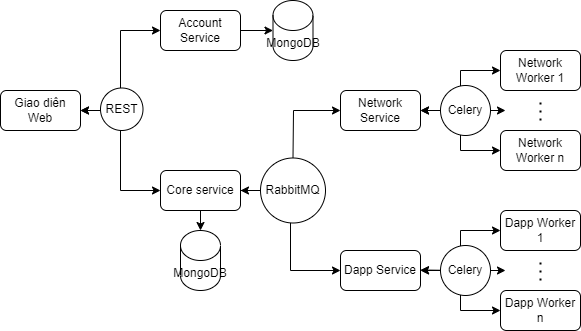
\includegraphics[width=0.75\linewidth]{Hinhve/DoAn-KienTrucTongQuan.drawio.png}
    \caption{Tổng quan các dịch vụ của hệ thống}
    \label{fig:overal_architecture}
\end{figure}

Hình \ref{fig:overal_architecture} mô tả tổng quan các dịch vụ trong hệ thống.
Các dịch vụ này bao gồm:

\begin{itemize}
    \item \textbf{Giao diện web:} Giao diện web người dùng sử dụng để tương tác với hệ thống.
    \item \textbf{Account service:} Dịch vụ quản lý tài khoản người dùng. Dịch vụ này sở hữu một cơ sở dữ liệu riêng biệt.
    \item \textbf{Core Service:} Dịch vụ cung cấp các chức năng chính. Dịch vụ này sẽ tương tác với Network và Dapp Service để hoàn thành yêu cầu người dùng. Dịch vụ này sở hữu một cơ sở dữ liệu riêng biệt.
    \item \textbf{Network service:} Dịch vụ xử lý các yêu cầu liên quan đến triển khai và quản lý mạng Hyperledger Fabric thông qua các Network Worker.
    \item \textbf{Network Worker:} Đơn vị trực tiếp thực hiện các tác vụ liên quan đến triển khai và quản lý mạng.
    \item \textbf{Dapp service:} Dịch vụ xử lý các yêu cầu liên quan đến triển khai và quản lý ứng dụng phi tập trung thông qua các Dapp Worker.
    \item \textbf{Dapp Worker:} Đơn vị trực tiếp thực hiện các tác vụ liên quan đến triển khai và quản lý ứng dụng phi tập trung.
\end{itemize}

Người dùng tương tác với Account và Core Service thông qua REST API. Account
service xử lý các yêu cầu liên quan đến tài khoản người dùng (đăng ký, đăng
nhập, xác thực). Core Service xử lý các yêu cầu liên quan đến mạng chuỗi khối
và ứng dụng phi tập trung. Core Service sẽ giao tiếp với Network và Dapp
Service thông qua RabbitMQ. Để xử lý các tác vụ mạng và ứng dụng nhận từ Core
service, hai service này sẽ thực hiện quản lý phân chia công việc cho các
Worker thông qua Celery.

\subsection{Kiến trúc tổng quan cơ sở dữ liệu}

\begin{figure}[H]
    \centering
    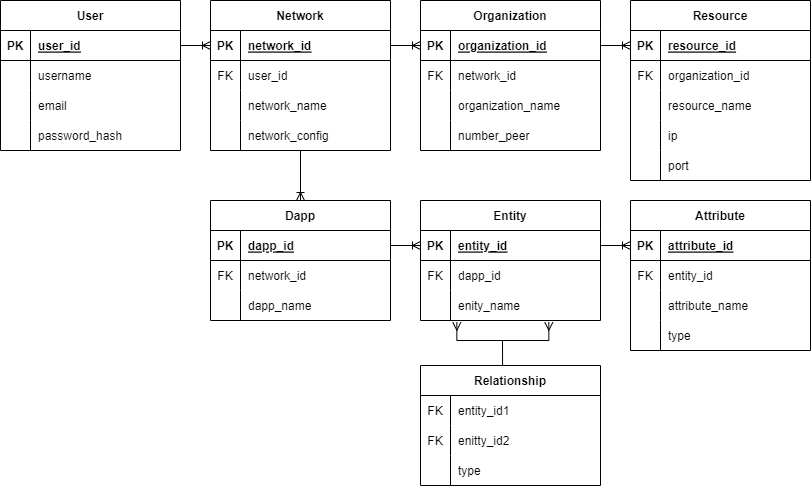
\includegraphics[width=0.75\linewidth]{Hinhve/DoAn-CSDLTongQuan.drawio.png}
    \caption{Cơ sở dữ liệu tổng quan}
    \label{fig:overal_database}
\end{figure}

Hình \ref{fig:overal_database} mô tả về thiết kế cơ sở dữ liệu cho các dịch vụ.
Với kiến trúc Microservices, các bảng sẽ được quản lý bởi nhiều dịch vụ.

Account service quản lý người dùng (User).

Core Service quản lý mạng (Network), tổ chức (Organization) và node ngoài
(Resource). Một người dùng có nhiều mạng và một mạng có nhiều tổ chức. Mỗi một
node ngoài sẽ thuộc về 1 tổ chức. Ngoài ra một mạng có nhiều ứng dụng phi tập
trung (Dapp). Cấu trúc của ứng dụng phi tập trung được định nghĩa thông qua các
thực thể (Entity), những thuộc tính (Attribute) của thực thể và quan hệ
(Relationship) giữa các thực thể.

Chi tiết thiết kế cơ sở dữ liệu cho từng dịch vụ sẽ được trình bày trong các
mục thiết kế chi tiết dịch vụ tương ứng tiếp theo.

\section{Thiết kế chi tiết}

\subsection{Thiết kế giao diện}

Thiết kế các màn hình chính cho giao diện của hệ thống sẽ được trình bày trong
phần này. Kích thước màn hình mà giao diện của hệ thống hướng đến là 16:9 cùng
độ phân giải được sử dụng là 1920 x 1080. Kích thước và độ phân giải này hiện
rất phổ biến hiện nay và thường được dùng cho màn hình máy tính, laptop.

\begin{figure}[H]
    \centering
    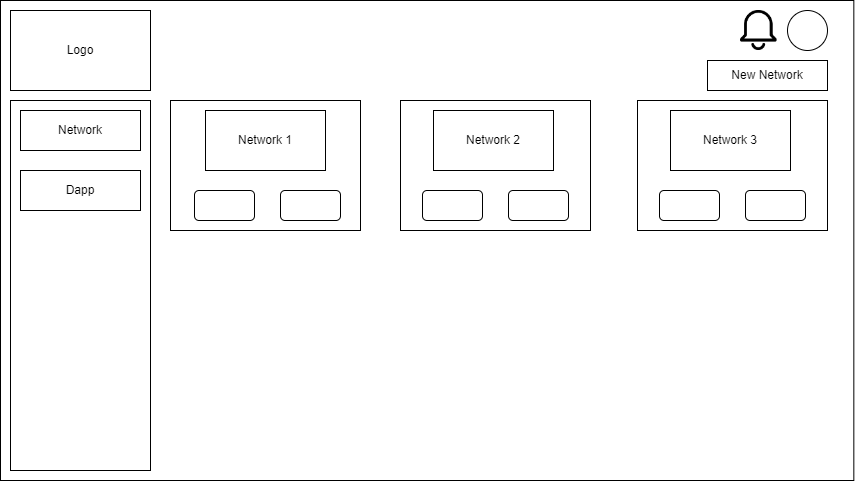
\includegraphics[width=0.75\linewidth]{Hinhve/DoAn-ScreenNetworks.drawio.png}
    \caption{Màn hình danh sách mạng}
    \label{fig:screenNetworks}
\end{figure}

Hình \ref{fig:screenNetworks} mô tả màn hình danh sách các mạng của người dùng.
Màn hình này sẽ hiện thị thông tin tổng quan về các mạng của người dùng, cùng
với đó là nút "New network" để tạo một mạng mới

\begin{figure}[H]
    \centering
    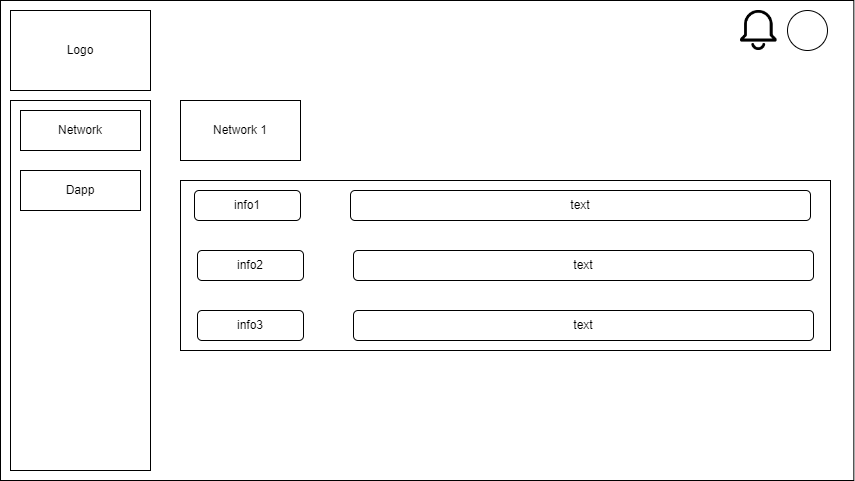
\includegraphics[width=0.75\linewidth]{Hinhve/DoAn-ScreenNetworkDetail.drawio.png}
    \caption{Màn hình thông tin mạng}
    \label{fig:screenNetworkDetail}
\end{figure}

Hình \ref{fig:screenNetworkDetail} mô tả màn hình chi tiết thông tin một mạng
của người dùng.

\begin{figure}[H]
    \centering
    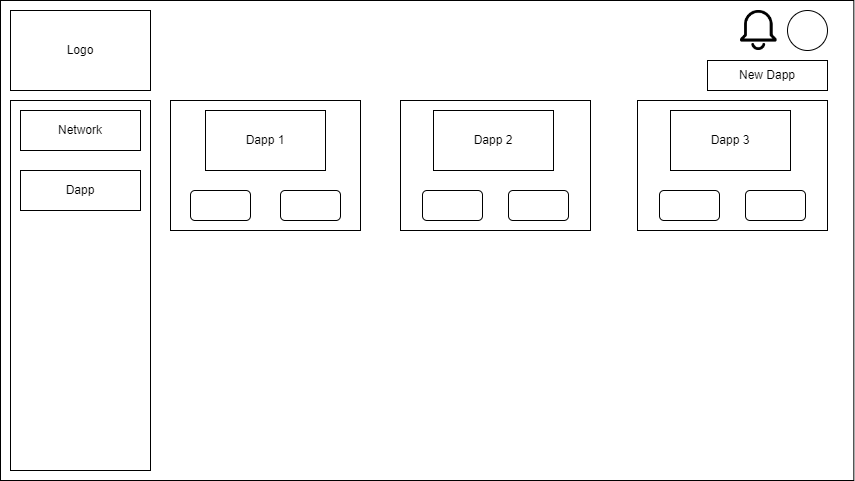
\includegraphics[width=0.75\linewidth]{Hinhve/DoAn-ScreenDapps.drawio.png}
    \caption{Màn hình danh sách ứng dụng}
    \label{fig:screenDapps}
\end{figure}

Hình \ref{fig:screenDapps} mô tả màn hình danh sách các ứng dụng của người
dùng. Về cơ bản, màn hình này có cấu trúc tương tụ với màn hình danh sách mạng
của người dùng.

\begin{figure}[H]
    \centering
    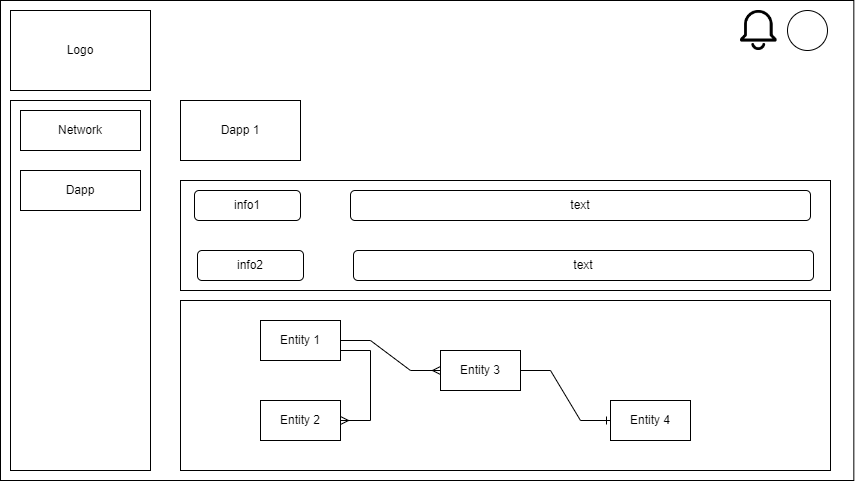
\includegraphics[width=0.75\linewidth]{Hinhve/DoAn-ScreenDappDetail.drawio.png}
    \caption{Màn hình thông tin ứng dụng}
    \label{fig:screenDappDetail}
\end{figure}

Hình \ref{fig:screenDappDetail} mô tả màn hình chi tiết thông tin một ứng dụng
phi tập trung của người dùng. Ngoài thông tin, chi tiết về cấu trúc của ứng
dụng được hiện thị trực quan thông qua một biểu đồ cơ sở dữ liệu quan hệ.

\begin{figure}[H]
    \centering
    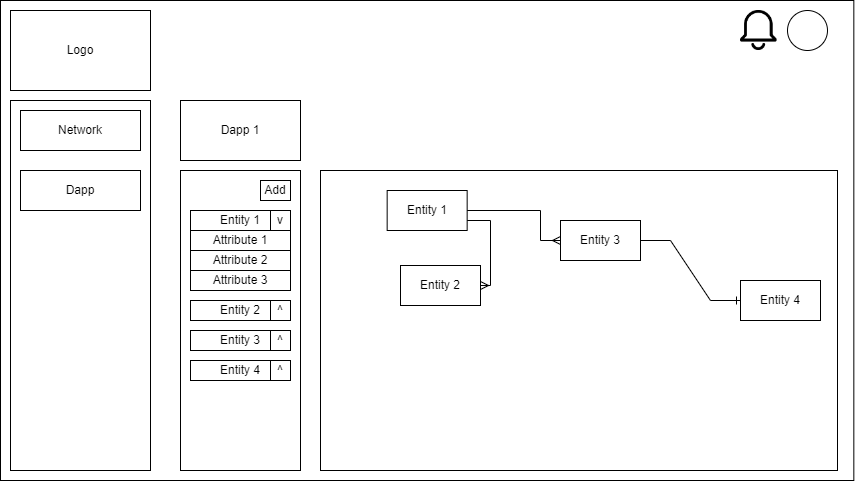
\includegraphics[width=0.75\linewidth]{Hinhve/DoAn-ScreenDappCreate.drawio.png}
    \caption{Màn hình tạo ứng dụng}
    \label{fig:screenDappCreate}
\end{figure}

Hình \ref{fig:screenDappDetail} mô tả màn hình tạo ứng dụng phi tập trung. Cấu
trúc của ứng dụng được định nghĩa theo sơ đồ cơ sở dữ liệu quan hệ. Hệ thống sẽ
cung cấp một giao diện để người dùng định nghĩa cấu trúc này một cách trực quan
nhất. Người dùng có thể tạo và định nghĩa các thuộc tính cho các thực thể với
thanh "Control". Tiếp đến sẽ thiết kế các quan hệ cho các thực thể bằng cách
tương tác với bảng "Overview".

\subsection{Thiết kế Account Service}

\subsubsection{Biểu đồ lớp}

\begin{figure}[H]
    \centering
    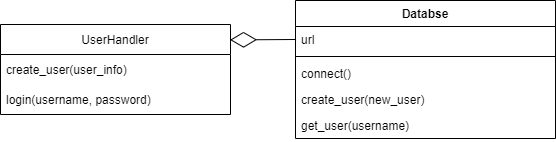
\includegraphics[width=0.75\linewidth]{Hinhve/DoAn-ClassAccountService.drawio.png}
    \caption{Biểu đồ lớp Account Service}
    \label{fig:classAccountService}
\end{figure}

Hình \ref{fig:classAccountService} mô tả biểu đồ lớp của Account service. Chi
tiết các lớp được mô tả ở Bảng \ref{tab:classAccountService}

\begin{longtable}{|p{0.175\textwidth}|p{0.175\textwidth}|p{0.2625\textwidth}|p{0.2625\textwidth}|}
    \caption{Mô tả chi tiết các lớp của Account service}
    \label{tab:classAccountService}                                                                                                                                                                                                \\
    \hline
    Tên lớp                                       & Mô tả lớp                                                         & Tên thuộc tính/ phương thức & Mô tả thuộc tính/ phương thức                                                \\ \hline
    \multirow[t]{2}{0.175\textwidth}{UserHandler} & \multirow[t]{2}{0.175\textwidth}{Xử lý các yêu cầu thông qua API} & create\_user(user\_info)    & Tạo một user mới với thông tin tương ứng với user\_info                      \\ \hline
                                                  &                                                                   & login(username, password)   & Đăng nhập người dùng vào hệ thống. Trả về JWT Token nếu đăng nhập thành công \\ \hline
    \multirow[t]{4}{0.175\textwidth}{Database}    & \multirow[t]{4}{0.175\textwidth}{Tương tác với cơ sở dữ liệu}     & url                         & Đường dẫn để kết nối tới cơ sở dữ liệu                                       \\ \cline{3-4}
                                                  &                                                                   & connect()                   & Kết nối tới cơ sở dữ liệu                                                    \\ \cline{3-4}
                                                  &                                                                   & create\_user(new\_user)     & Tạo một người dùng mới trong cơ sở dữ liệu                                   \\ \cline{3-4}
                                                  &                                                                   & get\_user(user\_info)       & Đọc thông tin về về người dùng từ cơ sở dữ liệu                              \\ \hline
\end{longtable}

\subsubsection{Thiết kế cơ sở dữ liệu}

Thiết kế chi tiết cơ sở dữ liệu cho Account Service được trình bày ở Bảng
\ref{tab:dbAccountService}

\begin{longtable}{|p{0.175\textwidth}|p{0.175\textwidth}|p{0.175\textwidth}|p{0.35\textwidth}|}
    \caption{Chi tiết cơ sở dữ liệu của Account service}
    \label{tab:dbAccountService}                                                                                 \\
    \hline
    Collection                             & Tên trường     & Kiểu dữ liệu & Mô tả                               \\ \hline
    \multirow[t]{4}{0.175\textwidth}{User} & user\_id       & ObjectId     & ID của người dùng                   \\ \cline{2-4}
                                           & username       & String       & Tên của người dùng                  \\ \cline{2-4}
                                           & email          & String       & Email của người dùng                \\ \cline{2-4}
                                           & password\_hash & String       & Giá trị băm của mật khẩu người dùng \\ \hline
\end{longtable}

\subsection{Thiết kế Core Service}

\subsubsection{Biểu đồ lớp}

\begin{figure}[H]
    \centering
    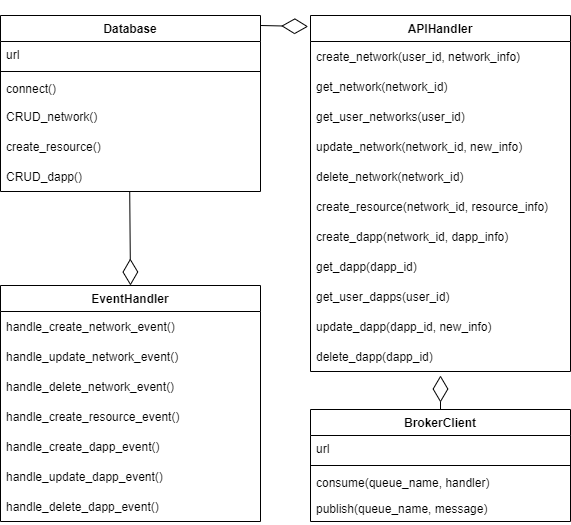
\includegraphics[width=0.75\linewidth]{Hinhve/DoAn-ClassCoreService.drawio.png}
    \caption{Biểu đồ lớp Core Service}
    \label{fig:classCoreService}
\end{figure}

Hình \ref{fig:classNetworkService} mô tả biểu đồ lớp của Core Service. Thông
tin các lớp được mô tả chi tiết ở Bảng \ref{tab:classCoreService}

\begin{longtable}{|p{0.175\textwidth}|p{0.175\textwidth}|p{0.2625\textwidth}|p{0.2625\textwidth}|}
    \caption{Mô tả chi tiết các lớp của Core Service}
    \label{tab:classCoreService}                                                                                                                                                                                                                                                                                           \\
    \hline
    Tên lớp                                        & Mô tả lớp                                                                          & Tên thuộc tính/ phương thức                                                       & Mô tả thuộc tính/ phương thức                                                                \\ \hline
    \multirow[t]{11}{0.175\textwidth}{ApiHandler}  & \multirow[t]{11}{0.175\textwidth}{Xử lý các yêu cầu thông qua API}                 & \hspace{0pt}create\_network\hspace{0pt}(user\_id, network\_info)                  & Tạo mới cho người dùng có ID user\_id một mạng có cấu hình network\_info                     \\ \cline{3-4}
                                                   &                                                                                    & \hspace{0pt}get\_network\hspace{0pt}(network\_id)                                 & Lấy thông tin về mạng có ID network\_id                                                      \\ \cline{3-4}
                                                   &                                                                                    & \hspace{0pt}get\_user\_networks\hspace{0pt}(user\_id)                             & Lấy thông tin về tất cả mạng của người dùng có ID user\_id                                   \\ \hline
                                                   &                                                                                    & \hspace{0pt}update\_network\hspace{0pt}(network\_id, new\_info)                   & Cập nhật mạng có ID network\_id cấu hình mới new\_info                                       \\ \cline{3-4}
                                                   &                                                                                    & \hspace{0pt}delete\_network\hspace{0pt}(network\_id)                              & Xóa mạng có ID network\_id                                                                   \\ \cline{3-4}
                                                   &                                                                                    & \hspace{0pt}create\_resource\hspace{0pt}(network\_id, resource\_info)             & Tạo một node ngoài có cấu hình resource\_info cho mạng có ID network\_id                     \\ \cline{3-4}
                                                   &                                                                                    & \hspace{0pt}create\_dapp\hspace{0pt}(network\_id, dapp\_info)                     & Tạo mới một ứng dụng phi tập trung có cấu hình dapp\_info cho mạng có ID network\_Id         \\ \cline{3-4}
                                                   &                                                                                    & \hspace{0pt}get\_dapp\hspace{0pt}(dapp\_id)                                       & Lấy thông tin về ứng dụng phi tập trung có ID dapp\_id                                       \\ \cline{3-4}
                                                   &                                                                                    & \hspace{0pt}get\_user\_dapps\hspace{0pt}(user\_id)                                & Lấy thông tin về tất cả ứng dụng phi tập trung của người dùng có ID user\_id                 \\ \cline{3-4}
                                                   &                                                                                    & \hspace{0pt}update\_dapp\hspace{0pt}(dapp\_id, new\_info)                         & Cập nhật mạng có ID dapp\_id cấu hình mới new\_info                                          \\ \cline{3-4}
                                                   &                                                                                    & \hspace{0pt}delete\_dapp\hspace{0pt}(dapp\_id)                                    & Xóa ứng dụng có ID dapp\_id                                                                  \\ \hline
    \multirow[t]{7}{0.175\textwidth}{EventHandler} & \multirow[t]{7}{0.175\textwidth}{Xử lý sự kiện được thông báo từ các dịch vụ khác} & \hspace{0pt}handle\_\hspace{0pt}create\_\hspace{0pt}network\_\hspace{0pt}event()  & Xử lý sự kiện mạng mới được tạo                                                              \\ \cline{3-4}
                                                   &                                                                                    & \hspace{0pt}handle\_\hspace{0pt}update\_\hspace{0pt}network\_\hspace{0pt}event()  & Xử lý sự kiện mạng được cập nhật                                                             \\ \cline{3-4}
                                                   &                                                                                    & \hspace{0pt}handle\_\hspace{0pt}delete\_\hspace{0pt}network\_\hspace{0pt}event()  & Xử lý sự kiện mạng được xóa                                                                  \\ \cline{3-4}
                                                   &                                                                                    & \hspace{0pt}handle\_\hspace{0pt}create\_\hspace{0pt}resource\_\hspace{0pt}event() & Xử lý sự kiện node ngoài được tạo                                                            \\ \hline
                                                   &                                                                                    & \hspace{0pt}handle\_\hspace{0pt}create\_\hspace{0pt}dapp\_\hspace{0pt}event()     & Xử lý sự kiện ứng dụng phi tập trung được tạo                                                \\ \cline{3-4}
                                                   &                                                                                    & \hspace{0pt}handle\_\hspace{0pt}update\_\hspace{0pt}dapp\_\hspace{0pt}event()     & Xử lý sự kiện ứng dụng phi tập trung được cập nhật                                           \\ \cline{3-4}
                                                   &                                                                                    & \hspace{0pt}handle\_\hspace{0pt}delete\_\hspace{0pt}dapp\_\hspace{0pt}event()     & Xử lý sự kiện ứng dụng phi tập trung bị xóa                                                  \\ \hline
    \multirow[t]{5}{0.175\textwidth}{Database}     & \multirow[t]{5}{0.175\textwidth}{Tương tác với cơ sở dữ liệu}                      & \hspace{0pt}url                                                                   & Đường dẫn kết nối tới cơ sở dữ liệu                                                          \\ \cline{3-4}
                                                   &                                                                                    & \hspace{0pt}connect\hspace{0pt}()                                                 & Kết nối tới cơ sở dữ liệu                                                                    \\ \cline{3-4}
                                                   &                                                                                    & \hspace{0pt}CRUD\_network\hspace{0pt}()                                           & Đọc ghi xóa sửa thông tin mạng trong cơ sở dữ liệu                                           \\ \cline{3-4}
                                                   &                                                                                    & \hspace{0pt}create\_resource\hspace{0pt}()                                        & Ghi thông tin node ngoài mới vào cơ sở dữ liệu                                               \\ \cline{3-4}
                                                   &                                                                                    & \hspace{0pt}CRUD\_dapp\hspace{0pt}()                                              & Đọc ghi xóa sủa thông tin ứng dụng phi tập trung trong cơ sở dữ liệu                         \\ \hline
    \multirow[t]{3}{0.175\textwidth}{BrokerClient} & \multirow[t]{3}{0.175\textwidth}{Tương tác với message broker}                     & \hspace{0pt}url                                                                   & Đường dẫn để kết nối tới message broker                                                      \\ \cline{3-4}
                                                   &                                                                                    & \hspace{0pt}consume\hspace{0pt}(queue\_name, handler)                             & Lắng nghe sự kiện từ hàng đợi queue\_name của message broker và xử lý xử kiện đó với handler \\ \cline{3-4}
                                                   &                                                                                    & \hspace{0pt}publish\hspace{0pt}(queue\_name, message)                             & Gửi một message tới hàng đợi queue\_name của message broker                                  \\ \hline
\end{longtable}

\subsubsection{Thiết kế cơ sở dữ liệu}

Thiết kế chi tiết cơ sở dữ liệu cho Core Service được trình bày ở Bảng
\ref{tab:dbCoreService}

% Please add the following required packages to your document preamble:
% \usepackage{multirow}

\begin{longtable}{|p{0.175\textwidth}|p{0.175\textwidth}|p{0.175\textwidth}|p{0.35\textwidth}|}
    \caption{Chi tiết cơ sở dữ liệu của Core Service}
    \label{tab:dbCoreService}                                                                                                     \\
    \hline
    Collection                                     & Tên trường         & Kiểu dữ liệu & Mô tả                                    \\ \hline
    \endhead
    \multirow[t]{4}{0.175\textwidth}{Network}      & network\_id        & ObjectId     & ID của mạng                              \\ \cline{2-4}
                                                   & user\_id           & ObjectId     & ID của người dùng sở hữu mạng            \\ \cline{2-4}
                                                   & network\_name      & String       & Tên của mạng                             \\ \cline{2-4}
                                                   & network\_config    & Object       & Cấu hình mạng                            \\ \hline
    \multirow[t]{4}{0.175\textwidth}{Organization} & organization\_id   & ObjectId     & ID của tổ chức                           \\ \cline{2-4}
                                                   & network\_id        & ObjectId     & ID của mạng mà tổ chức thuộc về          \\ \cline{2-4}
                                                   & organization\_name & String       & Tên tổ chức                              \\ \cline{2-4}
                                                   & number\_peer       & Number       & Số peer node trong tổ chức               \\ \hline
    \multirow[t]{5}{0.175\textwidth}{Resource}     & resource\_id       & ObjectId     & ID của node ngoài                        \\ \cline{2-4}
                                                   & organization\_id   & ObjectId     & ID của tổ chức mà node ngoài thuộc về    \\ \cline{2-4}
                                                   & resource\_name     & String       & Tên node ngoài                           \\ \cline{2-4}
                                                   & ip                 & String       & Địa chỉ IP của máy mà node ngoài sẽ chạy \\ \cline{2-4}
                                                   & port               &              & Cổng mạng của máy mà node ngoài sẽ chạy  \\ \hline
    \multirow[t]{3}{0.175\textwidth}{Dapp}         & dapp\_id           & ObjectId     & ID của ứng dụng                          \\ \cline{2-4}
                                                   & network\_id        & ObjectId     & ID của mạng mà ứng dụng thuộc về         \\ \cline{2-4}
                                                   & dapp\_name         & String       & Tên ứng dụng                             \\ \hline
    \multirow[t]{3}{0.175\textwidth}{Entity}       & entity\_id         & ObjectId     & ID của thực thể                          \\ \cline{2-4}
                                                   & dapp\_id           & ObjectId     & ID của ứng dụng mà thực thể thuộc về     \\ \cline{2-4}
                                                   & entity\_name       & String       & Tên ứng dụng                             \\ \hline
    \multirow[t]{4}{0.175\textwidth}{Attribute}    & attribute\_id      & ObjectId     & ID của thuộc tính                        \\ \cline{2-4}
                                                   & entity\_id         & ObjectId     & ID của thực thể mà thuộc tính thuộc về   \\ \cline{2-4}
                                                   & attribute\_name    & String       & Tên thuộc tính                           \\ \cline{2-4}
                                                   & type               & String       & Kiểu dữ liệu của thuộc tính              \\ \hline
    \multirow[t]{3}{0.175\textwidth}{Relationship} & entity\_id1        & ObjectId     & ID của thực thể đầu tiên                 \\ \cline{2-4}
                                                   & entity\_id2        & ObjectId     & ID của thực thể còn lại                  \\ \cline{2-4}
                                                   & type               & String       & Kiểu quan hệ                             \\ \hline
\end{longtable}

\subsection{Thiết kế Network Service}

\begin{figure}[H]
    \centering
    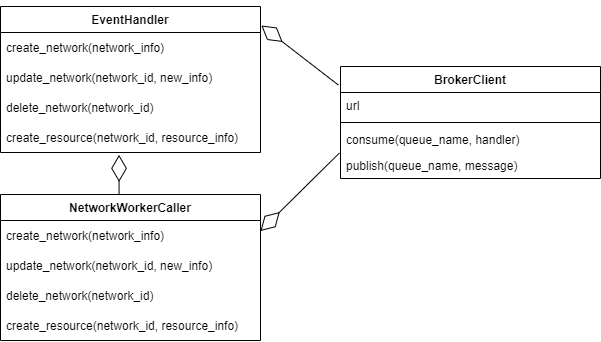
\includegraphics[width=0.75\linewidth]{Hinhve/DoAn-ClassNetworkService.drawio.png}
    \caption{Biểu đồ lớp Network Service}
    \label{fig:classNetworkService}
\end{figure}

Hình \ref{fig:classNetworkService} mô tả biểu đồ lớp của Network Service. Chi
tiết các lớp được mô tả ở Bảng \ref{tab:classNetworkService}

\begin{longtable}{|p{0.175\textwidth}|p{0.175\textwidth}|p{0.2625\textwidth}|p{0.2625\textwidth}|}
    \caption{Mô tả chi tiết các lớp của Network service}
    \label{tab:classNetworkService}                                                                                                                                                                                                                                                \\
    \hline
    Tên lớp                                                    & Mô tả lớp                                                                 & Tên thuộc tính/ phương thức                               & Mô tả thuộc tính/ phương thức                                             \\ \hline
    \endhead
    \multirow[t]{4}{0.175\textwidth}{\hspace{0pt}EventHandler} & \multirow[t]{4}{0.175\textwidth}{Xử lý yêu cầu từ Core Service}           & create\_network\hspace{0pt}(network\_info)                & Xử lý yêu cầu tạo mạng với cấu hình network\_info                         \\ \cline{3-4}
                                                               &                                                                           & update\_network\hspace{0pt}(network\_id, new\_info)       & Xử lý yều cầu cập nhật mạng có ID network\_id với thông tin mới new\_info \\ \cline{3-4}
                                                               &                                                                           & delete\_network\hspace{0pt}(network\_id)                  & Xử lý yêu cầu xóa mạng có ID network\_id                                  \\ \cline{3-4}
                                                               &                                                                           & create\_resource\hspace{0pt}(resource\_info)              & Xử lý yêu cầu tạo node ngoài có cấu hình resource\_info                   \\ \hline
    \multirow[t]{4}{0.175\textwidth}{\hspace{0pt}WorkerCaller} & \multirow[t]{4}{0.175\textwidth}{Yêu cầu Network Worker thực hiện tác vụ} & create\_network\hspace{0pt}(network\_info)                & Yêu cầu tạo mạng với cấu hình network\_info                               \\ \cline{3-4}
                                                               &                                                                           & update\_network\hspace{0pt}(network\_id, new\_info)       & Yêu cầu cập nhật mạng có ID network\_id với thông tin mới new\_info       \\ \hline
                                                               &                                                                           & delete\_network\hspace{0pt}(network\_id)                  & Yêu cầu xóa mạng có ID network\_id                                        \\ \cline{3-4}
                                                               &                                                                           & create\_resource\hspace{0pt}(resource\_info)              & Yêu cầu tạo node ngoài có cấu hình resource\_info                         \\ \hline
    BrokerClient                                               & Tương tác với message broker                                              & \multicolumn{2}{p{0.525\textwidth}|}{Tương tự Core Service}                                                                             \\ \hline
\end{longtable}

\subsection{Thiết kế Network Worker}

\begin{figure}[H]
    \centering
    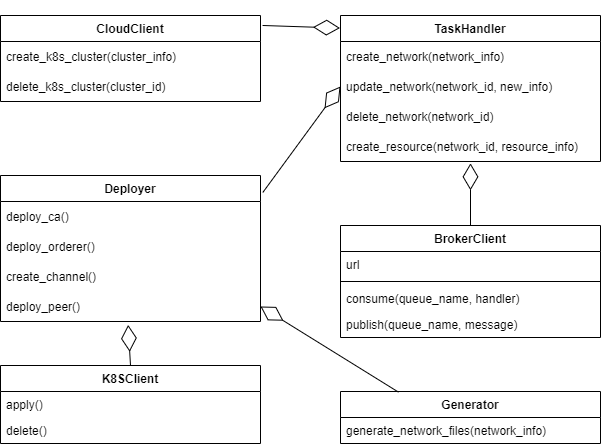
\includegraphics[width=0.5\linewidth]{Hinhve/DoAn-ClassNetworkWorker.drawio.png}
    \caption{Biểu đồ lớp Network Worker}
    \label{fig:classNetworkWorker}
\end{figure}

Hình \ref{fig:classNetworkWorker} mô tả biểu đồ lớp của Network Worker. Chi
tiết các lớp được mô tả ở Bảng \ref{tab:classNetworkWorker}

\begin{longtable}{|p{0.175\textwidth}|p{0.175\textwidth}|p{0.2625\textwidth}|p{0.2625\textwidth}|}
    \caption{Mô tả chi tiết các lớp của Network Worker}
    \label{tab:classNetworkWorker}                                                                                                                                                                                                                                          \\
    \hline
    Tên lớp                                       & Mô tả lớp                                                                 & Tên thuộc tính/ phương thức                                     & Mô tả thuộc tính/ phương thức                                             \\ \hline
    \endhead
    \multirow[t]{4}{0.175\textwidth}{TaskHandler} & \multirow[t]{4}{0.175\textwidth}{Xử lý yêu cầu từ Network Service}        & create\_network\hspace{0pt}(network\_info)                      & Xử lý yêu cầu tạo mạng với cấu hình network\_info                         \\ \hline
                                                  &                                                                           & update\_network\hspace{0pt}(network\_id, new\_info)             & Xử lý yều cầu cập nhật mạng có ID network\_id với thông tin mới new\_info \\ \cline{3-4}
                                                  &                                                                           & delete\_network\hspace{0pt}(network\_id)                        & Xử lý yêu cầu xóa mạng có ID network\_id                                  \\ \cline{3-4}
                                                  &                                                                           & create\_resource\hspace{0pt}(resource\_info)                    & Xử lý yêu cầu tạo node ngoài có cấu hình resource\_info                   \\ \hline
    \multirow[t]{2}{0.175\textwidth}{CloudClient} & \multirow[t]{2}{0.175\textwidth}{Tương tác với dịch vụ điện toán đám mây} & create\_k8s\_cluster\hspace{0pt}(cluster\_info)                 & Tạo một cụm Kubernetes                                                    \\ \cline{3-4}
                                                  &                                                                           & delete\_k8s\_cluster\hspace{0pt}(cluster\_id)                   & Xóa một cụm Kubernetes                                                    \\ \hline
    \multirow[t]{4}{0.175\textwidth}{Deployer}    & \multirow[t]{4}{0.175\textwidth}{Triển khai và quản lý mạng}              & deploy\_ca()                                                    & Triển khai Nhà cung cấp chứng chỉ số                                      \\ \cline{3-4}
                                                  &                                                                           & deploy\_orderer()                                               & Triển khai Orderer node                                                   \\ \cline{3-4}
                                                  &                                                                           & create\_channel()                                               & Tạo một kênh cho mạng                                                     \\ \cline{3-4}
                                                  &                                                                           & deploy\_peer()                                                  & Triển khai Peer node                                                      \\ \hline
    \multirow[t]{2}{0.175\textwidth}{K8SClient}   & \multirow[t]{2}{0.175\textwidth}{Tương tác với cụm Kubernetes}            & apply()                                                         & Thực hiện tác vụ tạo hoặc cập nhật trên cụm Kubernets                     \\ \cline{3-4}
                                                  &                                                                           & delete()                                                        & Thực hiện tác vụ tạo xóa trên cụm Kubernets                               \\ \hline
    Generator                                     & Tạo tệp tin                                                               & generate\_network\_\hspace{0pt}files\hspace{0pt}(network\_info) & Tạo các tập tin cho quá trình tạo mạng                                    \\ \hline
    BrokerClient                                  & Tương tác với message broker                                              & Tương tự Core Service                                           & Đường dẫn để kết nối tới message broker                                   \\ \hline
\end{longtable}

\subsection{Thiết kế Dapp Service}

\begin{figure}[H]
    \centering
    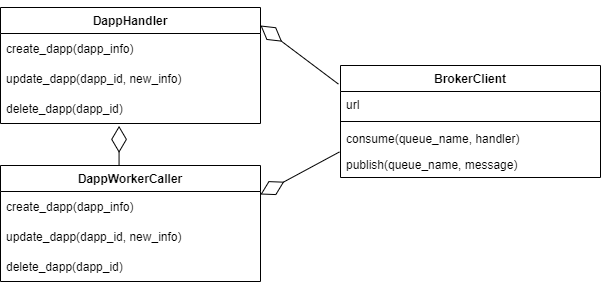
\includegraphics[width=0.75\linewidth]{Hinhve/DoAn-ClassDappService.drawio.png}
    \caption{Biểu đồ lớp Dapp Service}
    \label{fig:classDappService}
\end{figure}

Hình \ref{fig:classDappService} mô tả biểu đồ lớp của Dapp Service. Thông tin
các lớp được mô tả chi tiết ở Bảng \ref{tab:classDappService}

\begin{longtable}{|p{0.175\textwidth}|p{0.175\textwidth}|p{0.2625\textwidth}|p{0.2625\textwidth}|}
    \caption{Mô tả chi tiết các lớp của Dapp service}
    \label{tab:classDappService}                                                                                                                                                                                                                                     \\
    \hline
    Tên lớp                                        & Mô tả lớp                                                              & Tên thuộc tính/ phương thức                               & Mô tả thuộc tính/ phương thức                                              \\ \hline
    \endhead
    \multirow[t]{3}{0.175\textwidth}{EventHandler} & \multirow[t]{4}{0.175\textwidth}{Xử lý yêu cầu từ Core Service}        & create\_dapp\hspace{0pt}(dapp\_info)                      & Xử lý yêu cầu tạo ứng dụng với cấu hình dapp\_info                         \\ \cline{3-4}
                                                   &                                                                        & update\_dapp\hspace{0pt}(dapp\_id, new\_info)             & Xử lý yều cầu cập nhật ứng dụng có ID dapp\_id với thông tin mới new\_info \\ \cline{3-4}
                                                   &                                                                        & delete\_dapp\hspace{0pt}(dapp\_id)                        & Xử lý yêu cầu xóa ứng dụng có ID dapp\_id                                  \\ \hline
    \multirow[t]{3}{0.175\textwidth}{WorkerCaller} & \multirow[t]{4}{0.175\textwidth}{Yêu cầu Dapp Worker thực hiện tác vụ} & create\_dapp\hspace{0pt}(dapp\_info)                      & Yêu cầu tạo ứng dụng với cấu hình dapp\_info                               \\ \cline{3-4}
                                                   &                                                                        & update\_dapp\hspace{0pt}(dapp\_id, new\_info)             & Yêu cầu cập nhật ứng dụng có ID dapp\_id với thông tin mới new\_info       \\ \cline{3-4}
                                                   &                                                                        & delete\_dapp\hspace{0pt}(dapp\_id)                        & Yêu cầu xóa ứng dụng có ID dapp\_id                                        \\ \hline
    BrokerClient                                   & Tương tác với message broker                                           & \multicolumn{2}{p{0.525\textwidth}|}{Tương tự Core Service}                                                                              \\ \hline
\end{longtable}

\subsection{Thiết kế Dapp Worker}

\begin{figure}[H]
    \centering
    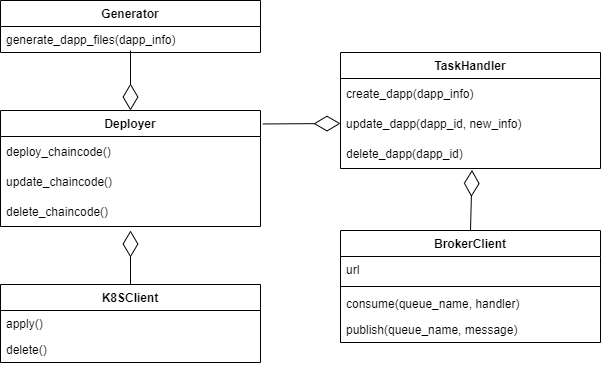
\includegraphics[width=0.75\linewidth]{Hinhve/DoAn-ClassDappWorker.drawio.png}
    \caption{Biểu đồ lớp Dapp Worker}
    \label{fig:classDappWorker}
\end{figure}

Hình \ref{fig:classDappWorker} mô tả biểu đồ lớp của Dapp Worker. Chi tiết các
lớp được mô tả ở Bảng \ref{tab:classDappWorker}

\begin{longtable}{|p{0.175\textwidth}|p{0.175\textwidth}|p{0.2625\textwidth}|p{0.2625\textwidth}|}
    \caption{Mô tả chi tiết các lớp của Dapp Worker}
    \label{tab:classDappWorker}                                                                                                                                                                                                                                 \\
    \hline
    Tên lớp                                       & Mô tả lớp                                                        & Tên thuộc tính/ phương thức                                 & Mô tả thuộc tính/ phương thức                                              \\ \hline
    \endhead
    \multirow[t]{3}{0.175\textwidth}{TaskHandler} & \multirow[t]{4}{0.175\textwidth}{Xử lý yêu cầu từ dapp Service}  & create\_dapp\hspace{0pt}(dapp\_info)                        & Xử lý yêu cầu tạo ứng dụng với cấu hình dapp\_info                         \\ \cline{3-4}
                                                  &                                                                  & update\_dapp\hspace{0pt}(dapp\_id, new\_info)               & Xử lý yều cầu cập nhật ứng dụng có ID dapp\_id với thông tin mới new\_info \\ \cline{3-4}
                                                  &                                                                  & delete\_dapp\hspace{0pt}(dapp\_id)                          & Xử lý yêu cầu xóa ứng dụng có ID dapp\_id                                  \\ \hline
    \multirow[t]{3}{0.175\textwidth}{Deployer}    & \multirow[t]{4}{0.175\textwidth}{Triển khai và quản lý ứng dụng} & deploy\_chaincode()                                         & Tạo và triển khai chaincode                                                \\ \cline{3-4}
                                                  &                                                                  & update\_chaincode()                                         & Cập nhật chaincode                                                         \\ \cline{3-4}
                                                  &                                                                  & delete\_chaincode()                                         & Xóa chaincode                                                              \\ \hline
    K8SClient                                     & Tương tác với cụm Kubernetes                                     & \multicolumn{2}{p{0.525\textwidth}|}{Tương tự Network Worker}                                                                              \\ \hline
    Generator                                     & Tạo tệp tin                                                      & generate\_dapp\_files\hspace{0pt}(dapp\_info)               & Tạo các tập tin cho quá trình tạo ứng dụng                                 \\ \hline
    BrokerClient                                  & Tương tác với message broker                                     & \multicolumn{2}{p{0.525\textwidth}|}{Tương tự Core Service}                                                                                \\ \hline
\end{longtable}

\subsection{Các luồng hoạt động chính}

Mục này sẽ mô tả trình tự tương tác giữa các dịch vụ trong hệ thống để thực
hiện yêu cầu từ người dùng.

\subsubsection{Tạo mạng}

\begin{figure}[H]
    \centering
    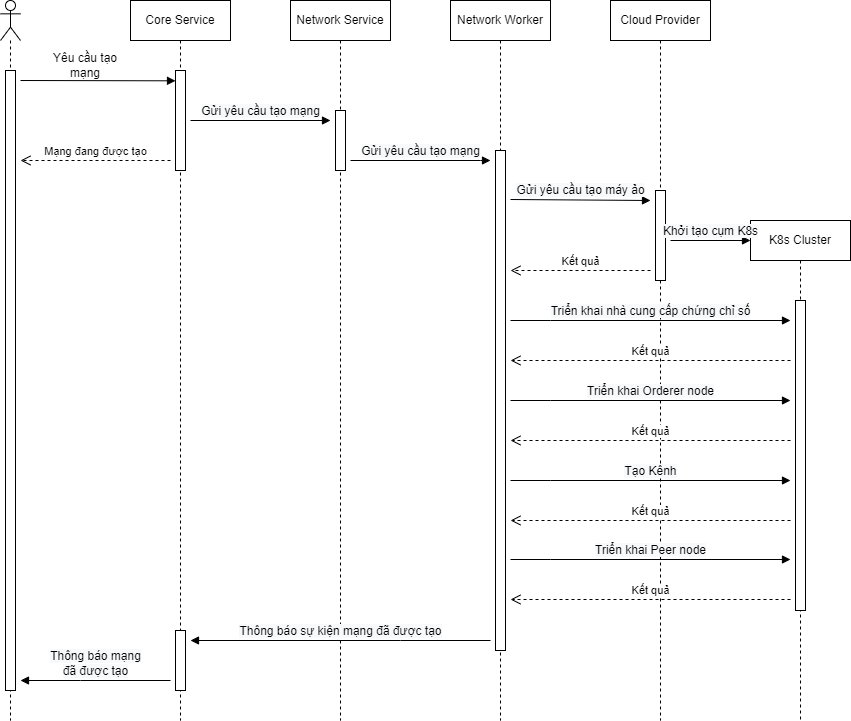
\includegraphics[width=0.75\linewidth]{Hinhve/DoAn-SeqCreateNetwork.drawio.png}
    \caption{Biểu đồ trình tự tạo mạng}
    \label{fig:seqCreateNetwork}
\end{figure}

Hình \ref{fig:seqCreateNetwork} mô tả luồng hoạt động của hệ thống để triển
khai một mạng chuỗi khối Hyperledger Fabric.

Trước hết, người dùng sử dụng giao diện để lựa chọn cấu hình cho mạng chuỗi
khối mới. Giao diện sẽ gửi thông tin mạng cần tạo về cho Core Service, dịch vụ
này sau đó sẽ gửi về thông báo rằng mạng đang được khởi tạo. Core Service sau
đó gửi yêu cầu tạo mạng tới Network Service. Network Service yêu cầu 1 trong số
các Network Worker thực hiện tác vụ tạo mạng.

Quá trình tạo mạng bắt đầu với việc Network Worker yêu cầu tạo một cụm máy ảo
tương ứng với cấu hình người dùng yêu cầu tới nhà cung cấp dịch vụ điện toán
đám mây. Sau khi một cụm Kubernetes mới đã được tạo, Network Worker sẽ tiến
hành triển khai một mạng Hyperledger Fabric lên trên cụm Kubernetes này. Bước
đầu tiên là triển khai các Nhà cung cấp chứng chỉ số. Tiếp đó, sử dụng chứng từ
số được tạo bởi các nhà cung cấp này, tiến hành triển khai Orderer Node. Tiếp
đến, thực hiện cấu hình và triển khai một kênh cho các tổ chức trong mạng theo
như yêu cầu người dùng đã gửi. Kế đến, các Peer node trực thuộc các tổ chức sẽ
được triển khai và tham gia vào kênh này. Bước cuối cùng trong quá trình tạo
mạng là triển khai một ứng dụng Explorer để có thể theo dõi các hoạt động trong
mạng.

Sau khi triển khai mạng hoàn tất, Network Worker thông báo với Core Service.
Core Service sẽ thông báo tới giao diện mạng đã triển khai thành công.

\subsubsection{Tạo ứng dụng phi tập trung}

\begin{figure}[H]
    \centering
    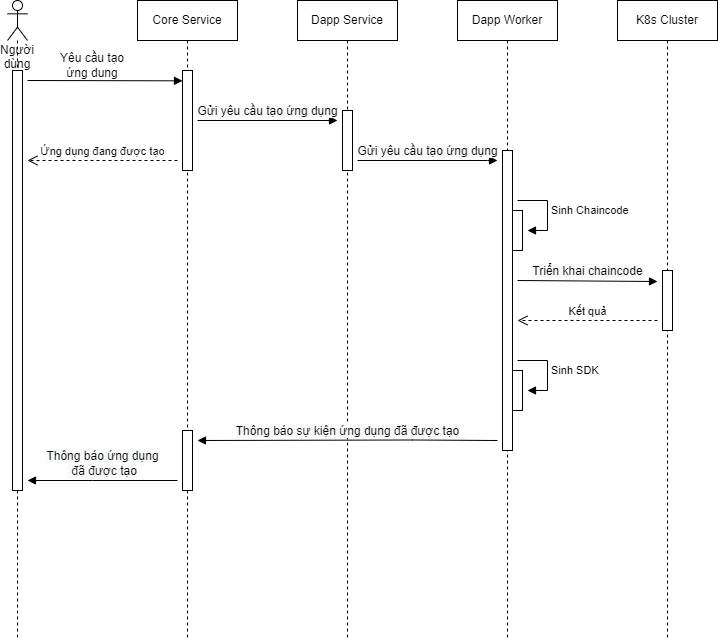
\includegraphics[width=0.75\linewidth]{Hinhve/DoAn-SeqCreateDapp.drawio.png}
    \caption{Biểu đồ trình tự tạo ứng dụng phi tập trung}
    \label{fig:seqCreateDapp}
\end{figure}

Hình \ref{fig:seqCreateDapp} mô tả luồng hoạt động của hệ thống để triển khai
một ứng dụng phi tập trung cho một mạng Hyperledger Fabric.

Tương tự như quá trình tạo mạng, người dùng gửi yêu cầu tới Core Service để tạo
một ứng dụng phi tập trung mới cho một mạng của người dùng. Thông qua giao
diện, cấu trúc của ứng dụng sẽ được định nghĩa với các thực thể sở hữu nhiều
thuộc tính có quan hệ với nhau. Yêu cầu tạo ứng dụng này sẽ được chuyển đến
Dapp Worker để tiến hành sinh và triển khai ứng dụng.

Từ cấu trúc mà người dùng yêu cầu, Dapp Worker sẽ sinh ra một chaincode tương
ứng. Chaincode này sẽ được triển khai lên cụm Kubernetes mà mạng chuỗi khối
đang chạy. Một SDK để tương tác với chaincode sau đó sẽ được tạo ra.

Sau khi triển khai ứng dụng thành công, Dapp Worker cũng sẽ gửi thông tin về
Core Service để dịch vụ này thông báo cho người dùng.

\subsubsection{Thêm node ngoài của người dùng vào mạng}

\begin{figure}[H]
    \centering
    \includegraphics[width=0.75\linewidth]{Hinhve/DoAn-seqAddNode.drawio.png}
    \caption{Biểu đồ trình tự thêm node ngoài vào mạng}
    \label{fig:seqAddNode}
\end{figure}

Hình \ref{fig:seqCreateNetwork} mô tả luồng hoạt động của hệ thống để thêm một
node ngoài vào mạng.

Người dùng gửi yêu cầu thêm node với cấu hình và địa chỉ IP mã node sẽ chạy tới
Core Service. Yêu cầu sẽ được chuyển tiếp tới Network Service. Dịch vụ này sẽ
tương tác với mạng đang chạy để tạo một định danh tương ứng cho node mới này.
Các tệp tin để khởi chạy node đó cũng sẽ được sinh ra.

Khi tệp tin đã được tạo người dùng sẽ nhận được thông báo từ Core Service.
Người dùng từ đó tải các tệp tin này về, khởi chạy node trên máy có địa chỉ IP
mà người dùng cung cấp lúc đầu. Node mới khi được khởi chạy sẽ tự động tham gia
vào mạng Hyperledger Fabric của người dùng.

\section{Xây dựng hệ thống}
\subsection{Thư viện và công cụ sử dụng}
Quá trình xây dựng và phát triển các dịch vụ trong hệ thống sử dụng những công
cụ và thư viện được nêu ở Bảng \ref{tab:toolsAndLib}.

\begin{longtable}{|p{0.2625\textwidth}|p{0.175\textwidth}|p{0.4375\textwidth}|}
    \caption{Danh sách thư viện và công cụ sử dụng}
    \label{tab:toolsAndLib}                                                                                                                  \\
    \hline
    \textbf{Mục đích}                                & \textbf{Công cụ}       & \textbf{Địa chỉ URL}                                         \\ \hline
    \endhead
    IDE lập trình                                    & Visual Code Studio     & \url{https://code.visualstudio.com/}                         \\ \hline
    Triển khai hệ thống                              & Docker                 & \url{https://www.docker.com}                                 \\ \hline
    Ngôn ngữ lập trình hệ thống                      & Python                 & \url{https://www.python.org/}                                \\ \hline
    Thư viện xây dựng Server http                    & aiohttp                & \url{https://pypi.org/project/aiohttp/}                      \\ \hline
    Thư viện kết nối tới RabbitMQ                    & aio\_pika              & \url{https://aio-pika.readthedocs.io/en/latest/}             \\ \hline
    Thư viện sinh tệp tin theo template              & Jinja                  & \url{https://jinja.palletsprojects.com/en/3.1.x/}            \\ \hline
    Tương tác với cụm Kubernetes                     & kubectl                & \url{https://kubernetes.io/docs/reference/kubectl/}          \\ \hline
    Tương tác với mạng Hyperledger Fabric            & Fabric CLI             & \url{https://github.com/hyperledger/fabric-cli}              \\ \hline
    Xây dựng CA cho mạng Hyperledger Fabric          & Fabric CA              & \url{https://github.com/hyperledger/fabric-ca}               \\ \hline
    Thư viện xây dựng giao diện web                  & ReactJS                & \url{https://ReactJS.org}                                    \\ \hline
    Thư viện quản lý trạng thái cho ứng dụng web     & EJ2 React Diagrams     & \url{https://redux.js.org}                                   \\ \hline
    Thư viện vẽ biểu đồ cơ sở dữ liệu quan hệ        & react-flow-renderer    & \url{https://www.npmjs.com/package/react-flow-renderer}      \\ \hline
    Ngôn ngữ lập trình cho SDK                       & Javascript             & \url{https://developer.mozilla.org/enUS/docs/Web/JavaScript} \\ \hline
    Thư viện sử dụng để xây dựng SDK                 & fabric-network         & \url{https://hyperledger.github.io/fabric-sdk-node/}         \\ \hline
    Xây dựng explorer cho mạng Hyperledger Fabric    & Hyperledger Explorer   & \url{https://github.com/hyperledger/blockchain-explorer}     \\ \hline
    Xây dựng hệ thống thông báo thông qua web socket & Notification-socket.io & \url{https://github.com/netbulls/notification-socket.io}     \\ \hline
\end{longtable}

\subsection{Minh họa các chức năng chính}

\begin{figure}[H]
    \centering
    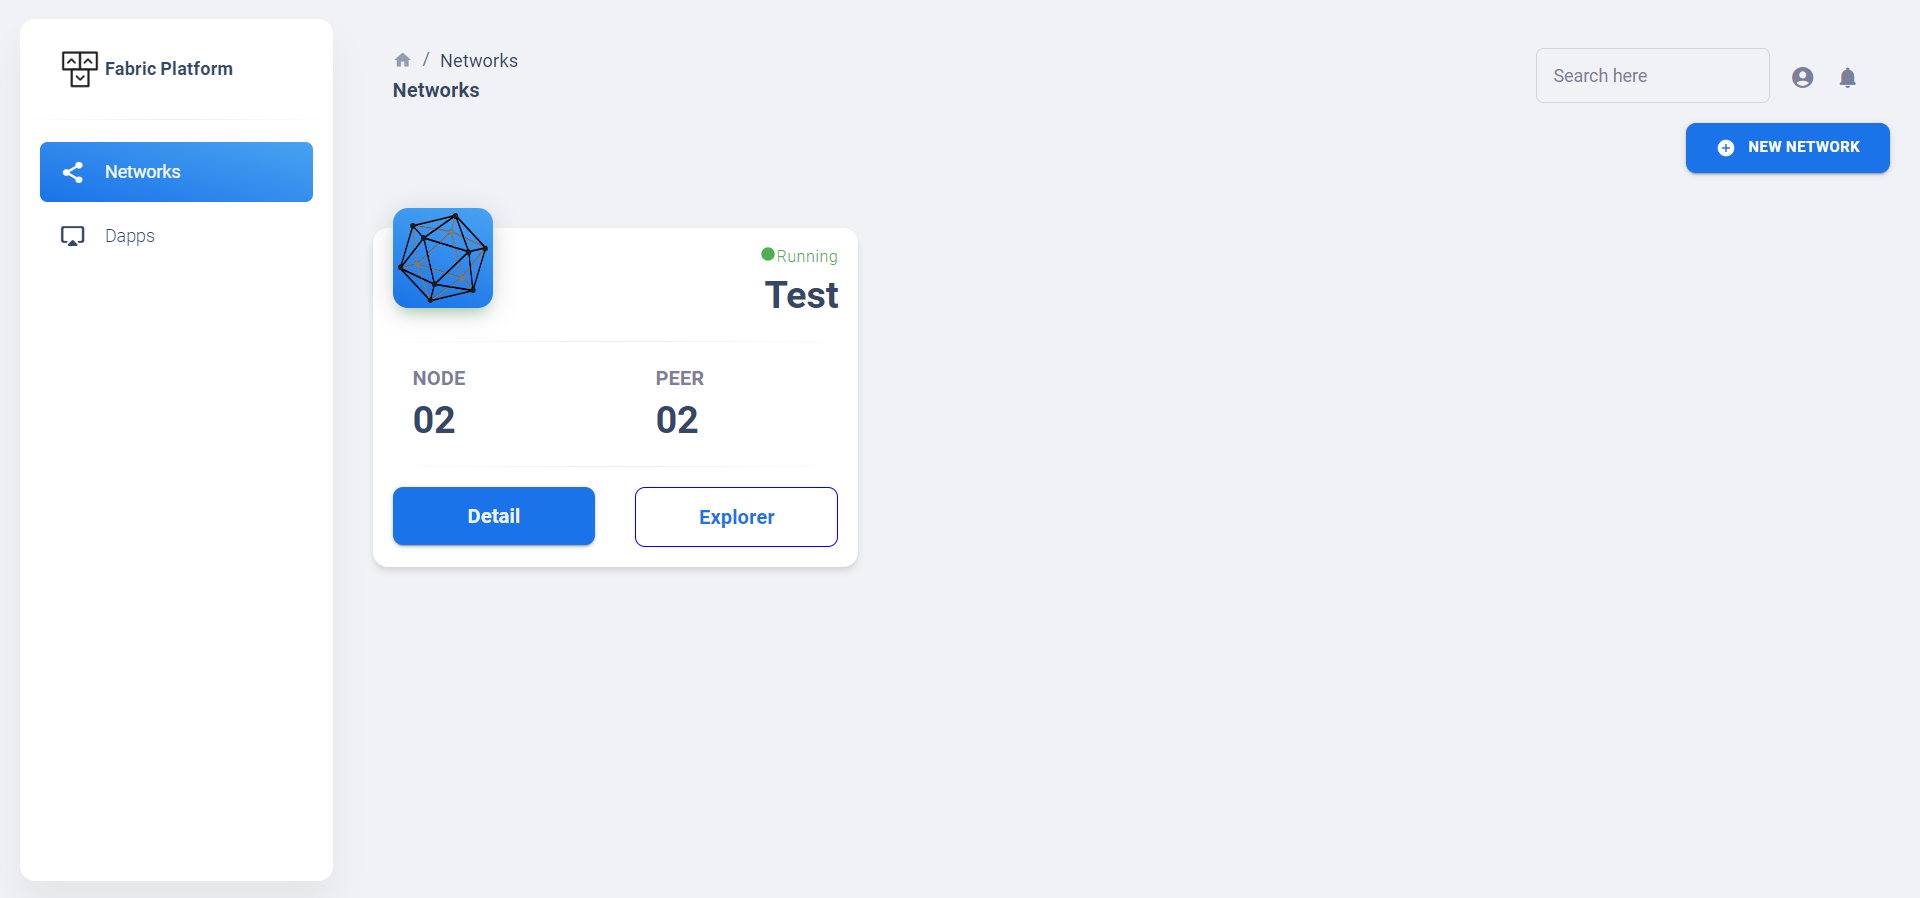
\includegraphics[width=0.75\linewidth]{Hinhve/DoAn-ResultNetworks.png}
    \caption{Màn hình danh sách mạng}
    \label{fig:ResultNetworks}
\end{figure}

Hình \ref{fig:ResultNetworks} mô tả màn hình danh sách mạng của người dùng. Tại
màn hình này, người dùng có thể thấy thông tin tổng quan nhất của các mạng cùng
với đó là truy cập vào Explorer của mạng. Người dùng có thể chọn "New network"
để tiến hành tạo mạng mới.

\begin{figure}[H]
    \centering
    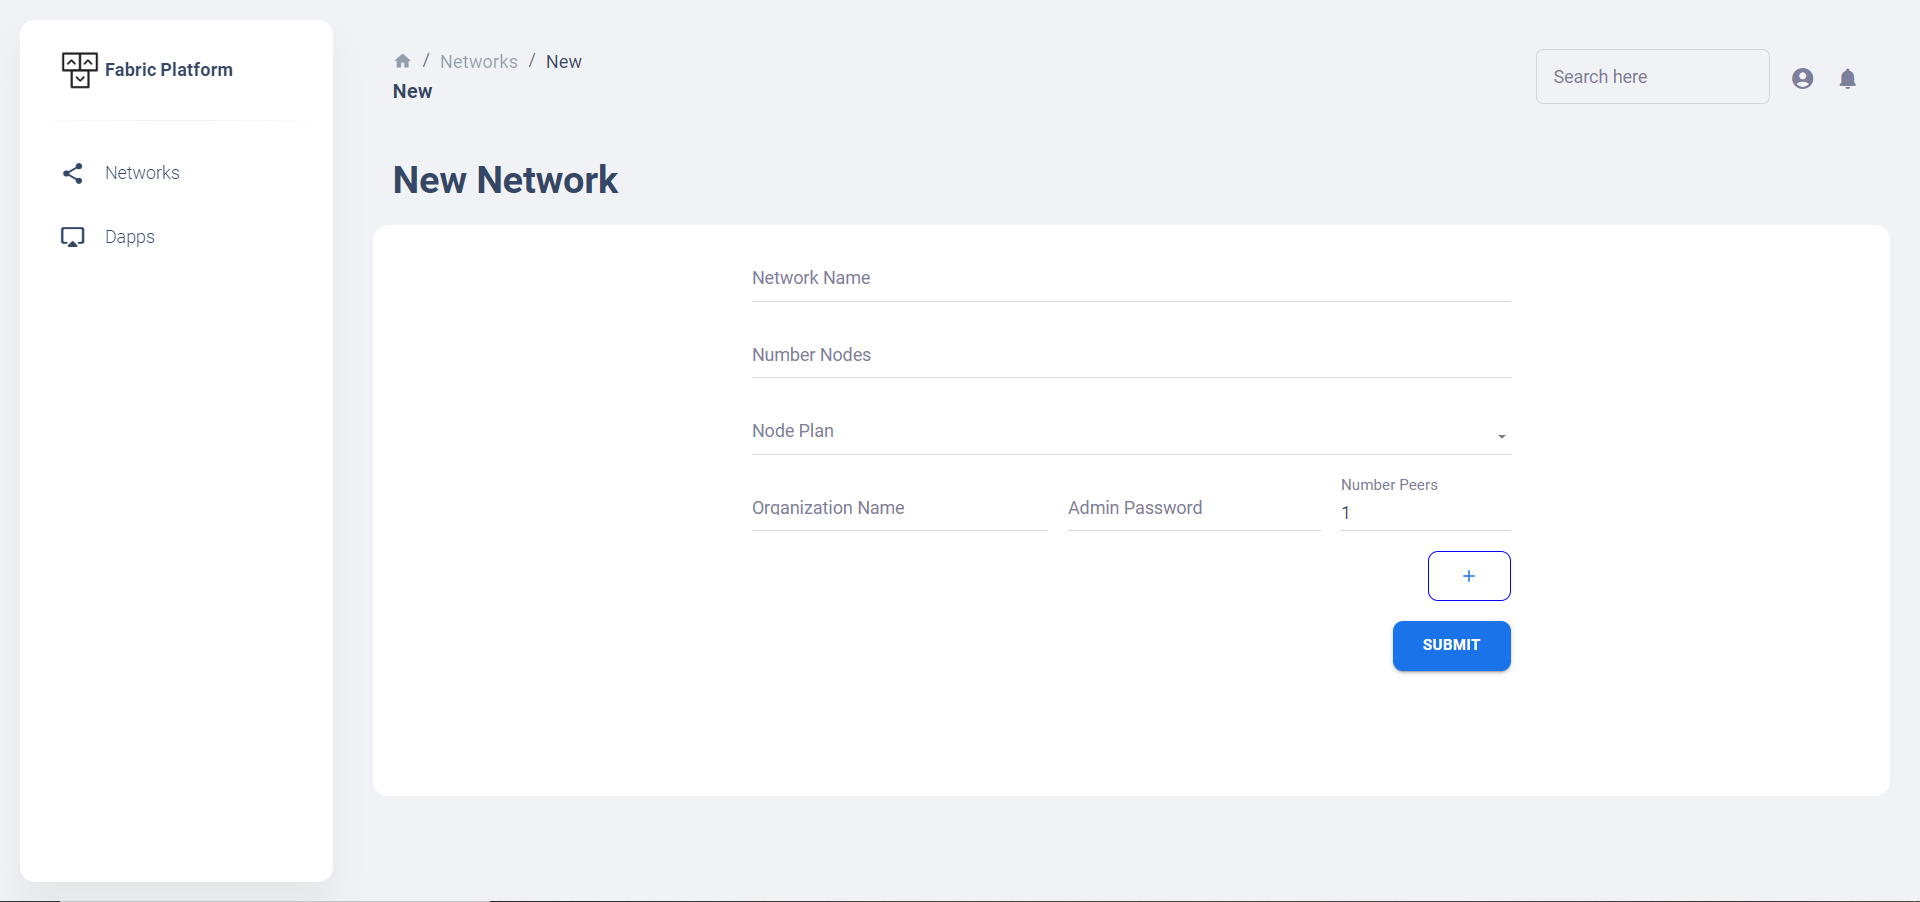
\includegraphics[width=0.75\linewidth]{Hinhve/DoAn-ResultNetworkNew.png}
    \caption{Màn hình tạo mạng mới}
    \label{fig:ResultNetworkNew}
\end{figure}

Hình \ref{fig:ResultNetworkNew} mô tả màn hình tạo mạng mới. Một mạng mới tương
ứng với thông tin người dùng nhập sẽ được tạo sau khi nhấn Submit.

\begin{figure}[H]
    \centering
    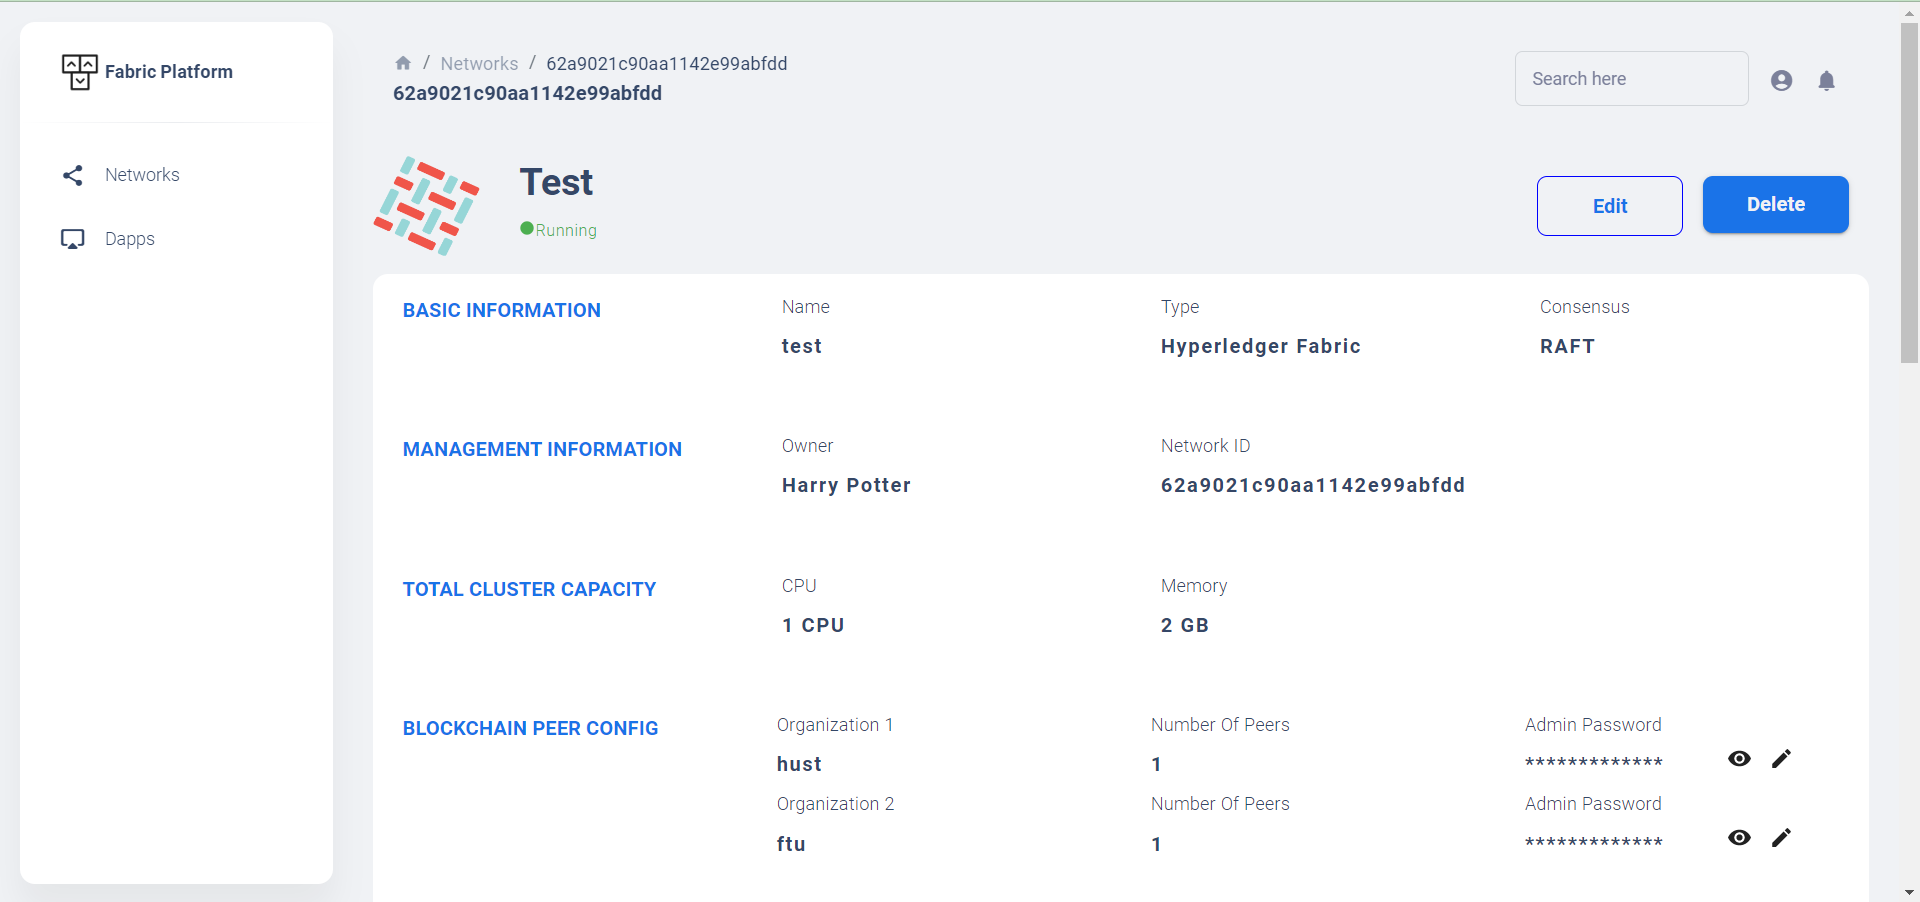
\includegraphics[width=0.75\linewidth]{Hinhve/DoAn-ResultNetworkDetail1.png}
    \caption{Màn hình thông tin mạng 1}
    \label{fig:ResultNetworkDetail1}
\end{figure}

\begin{figure}[H]
    \centering
    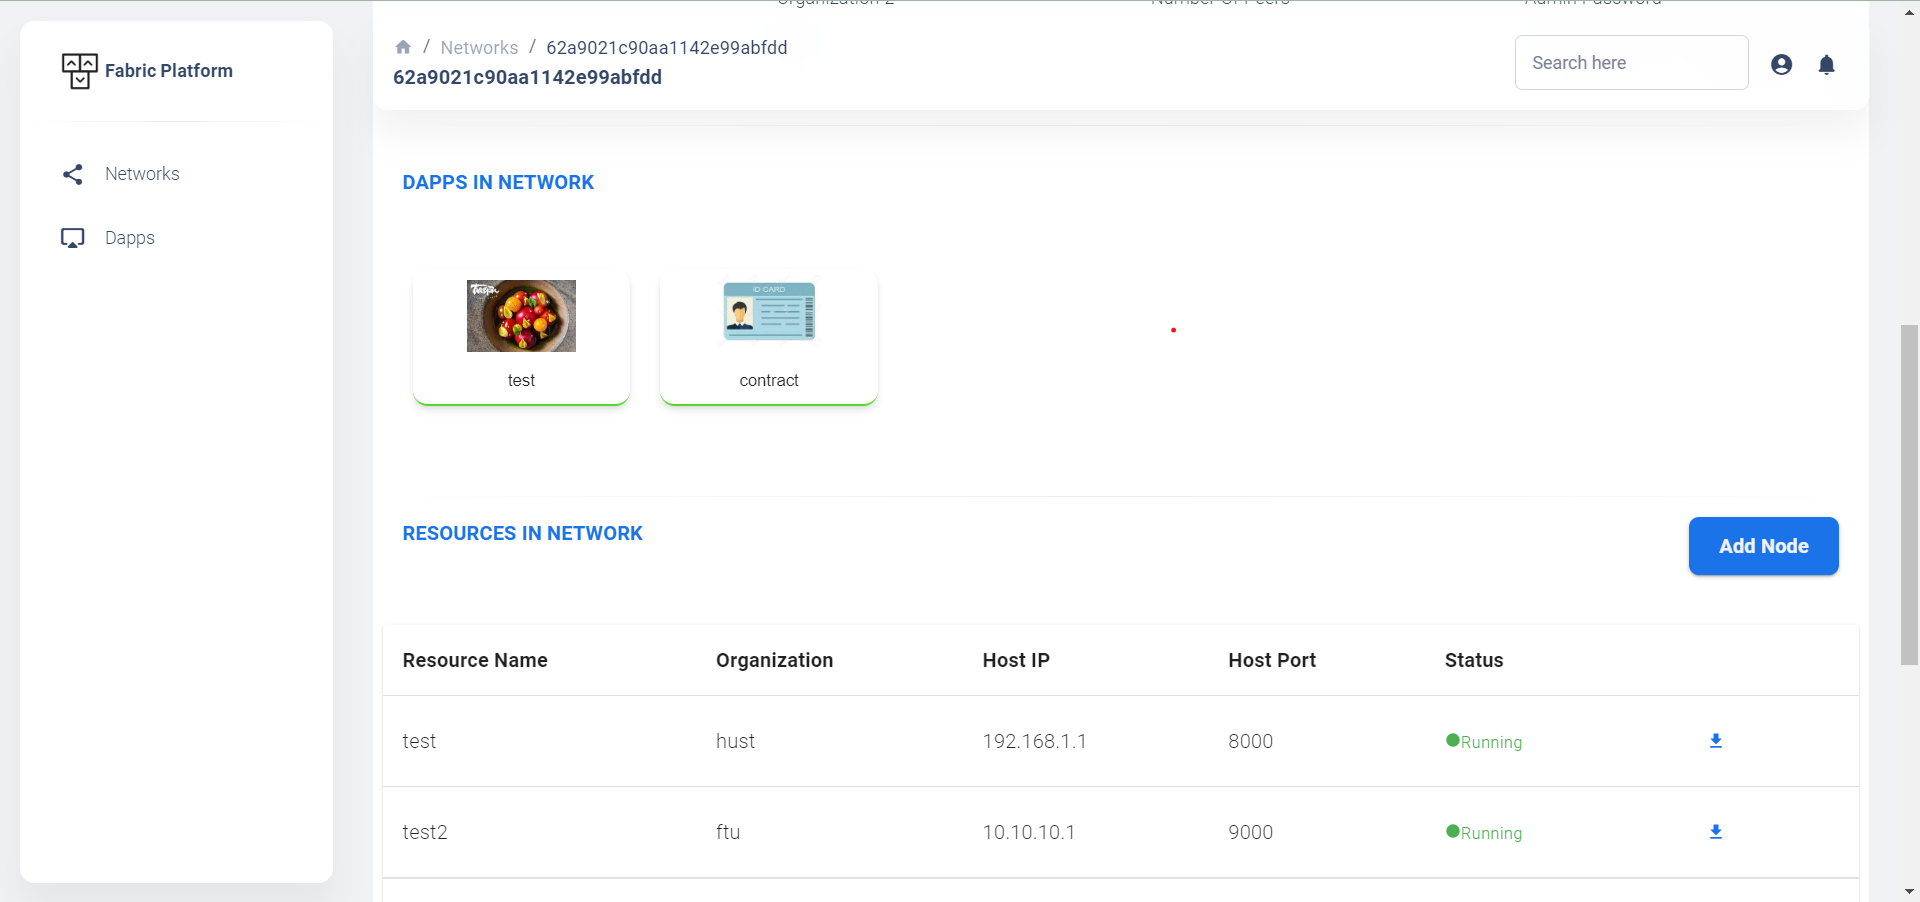
\includegraphics[width=0.75\linewidth]{Hinhve/DoAn-ResultNetworkDetail2.png}
    \caption{Màn hình thông tin mạng 2}
    \label{fig:ResultNetworkDetail2}
\end{figure}

Hình \ref{fig:ResultNetworkDetail1} và \ref{fig:ResultNetworkDetail2} mô tả màn
hình chi tiết thông tin của một mạng. Ngoài thông tin cơ bản của mạng, danh
sách ứng dụng và node ngoài thuộc về mạng cũng được hiện thị. Ngoài ra người
dùng có thể thực hiện xóa mạng thông qua nút "Delete", thêm tổ chức quá nút
"Edit" và thêm node ngoài thông qua nút "Add node".

\begin{figure}[H]
    \centering
    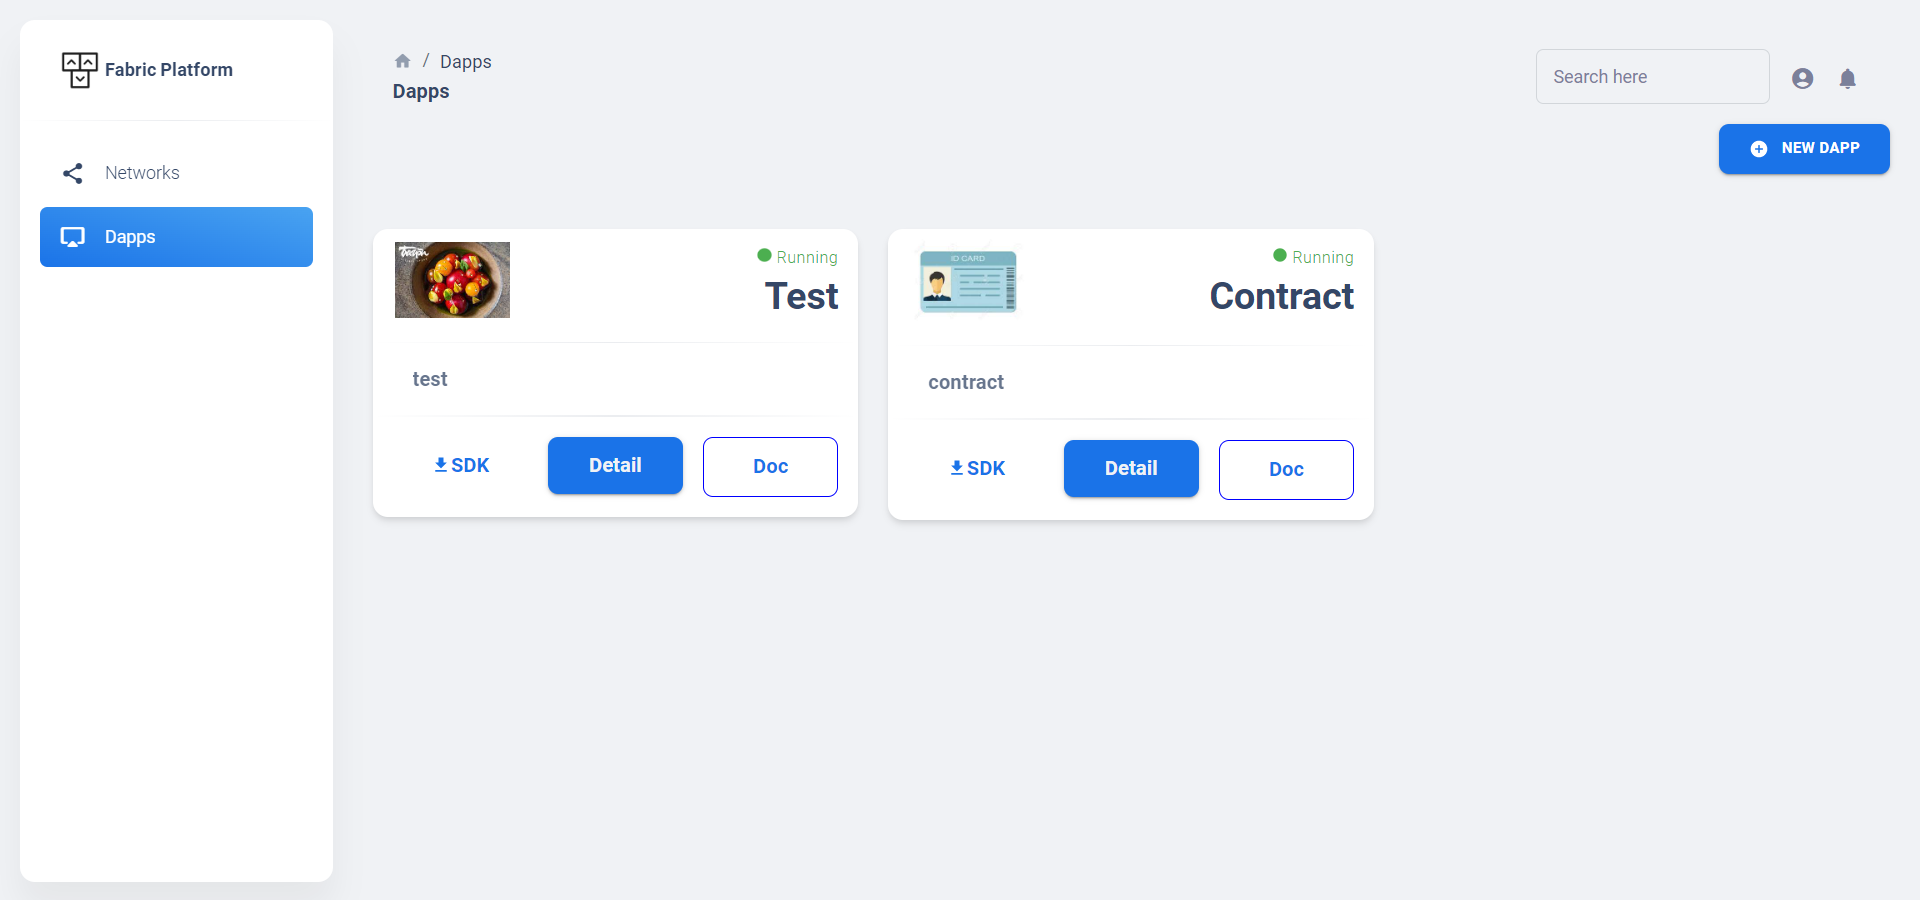
\includegraphics[width=0.75\linewidth]{Hinhve/DoAn-ResultDapps.png}
    \caption{Màn hình danh sách ứng dụng}
    \label{fig:ResultDapps}
\end{figure}

Hình \ref{fig:ResultDapps} mô tả danh sách ứng dụng phi tập trung của người
dùng. Ngoài thông tin cơ bản, người dùng có thể tải SDK và truy cập Tài liệu mô
tả SDK. Người dùng có thể tạo ứng dụng mới thông qua nút "New Dapp".

\begin{figure}[H]
    \centering
    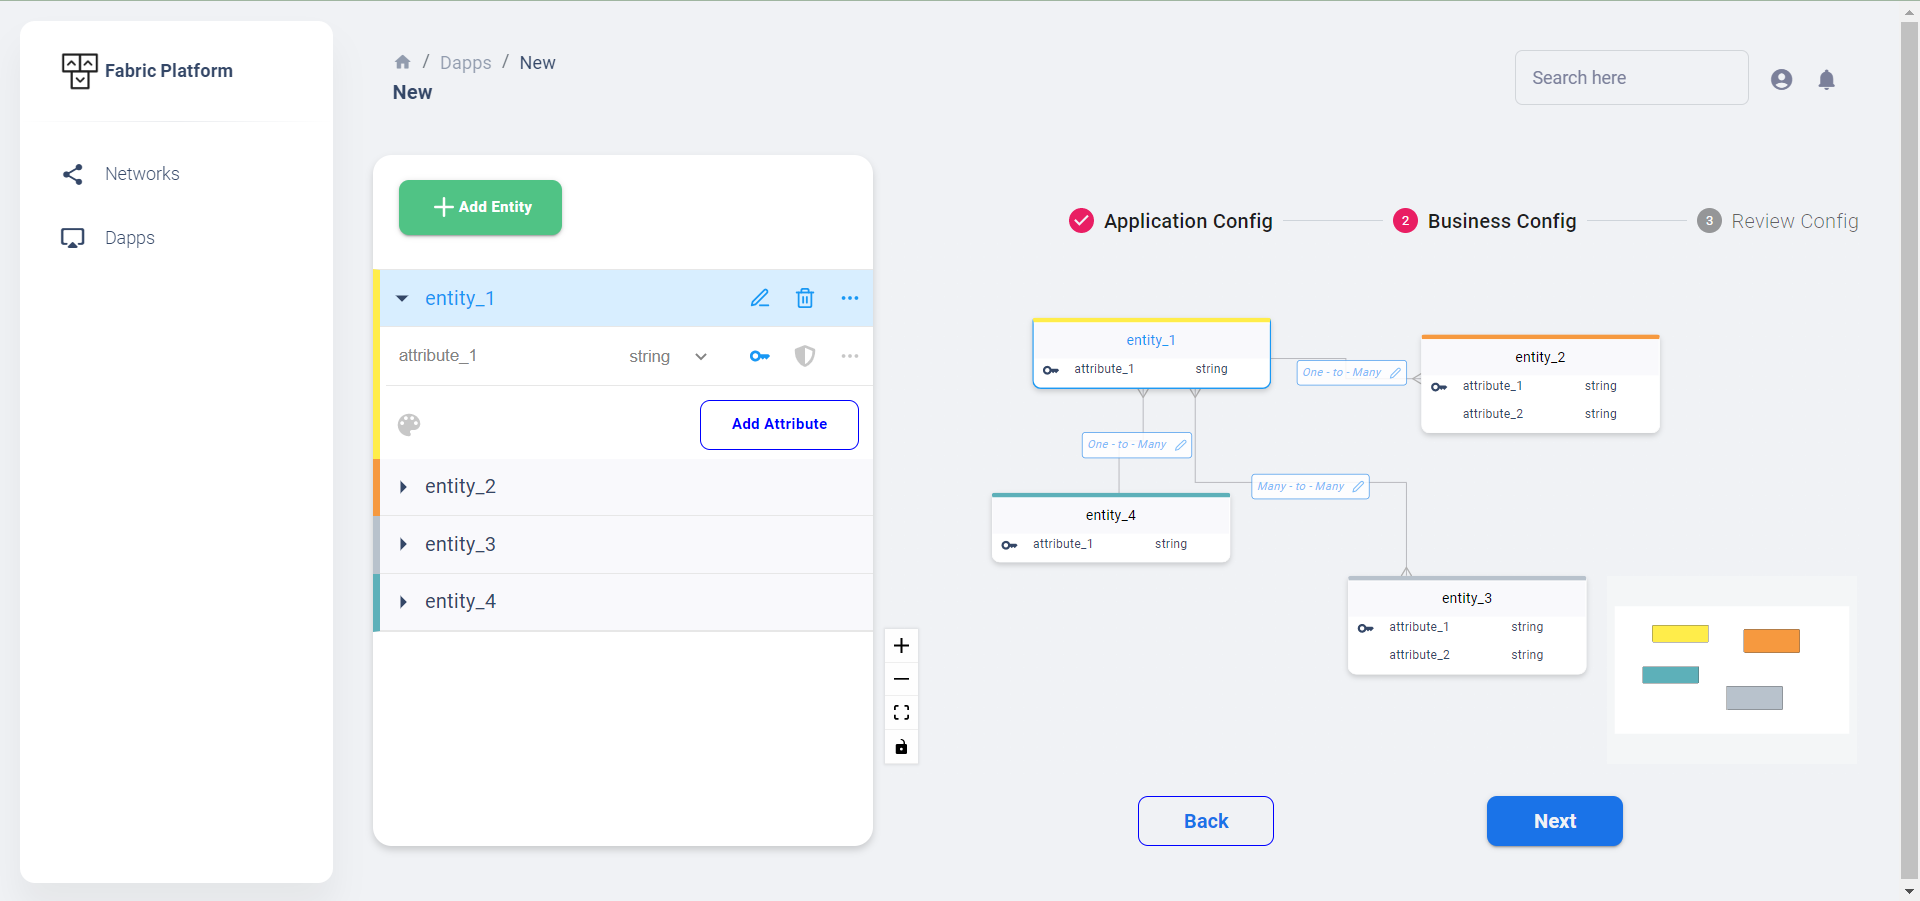
\includegraphics[width=0.75\linewidth]{Hinhve/DoAn-ResultDappCreate.png}
    \caption{Màn hình thiết kế cấu trúc ứng dụng}
    \label{fig:ResultDappCreate}
\end{figure}

Hình \ref{fig:ResultDappCreate} mô tả màn hình thiết kế cấu trúc ứng dụng phi
tập trung mới. Người dùng có thể tạo các thực thể với nhiều thuộc tính. Rồi kết
nối các thực thể này với nhau thông qua một giao diện kéo thả.

\begin{figure}[H]
    \centering
    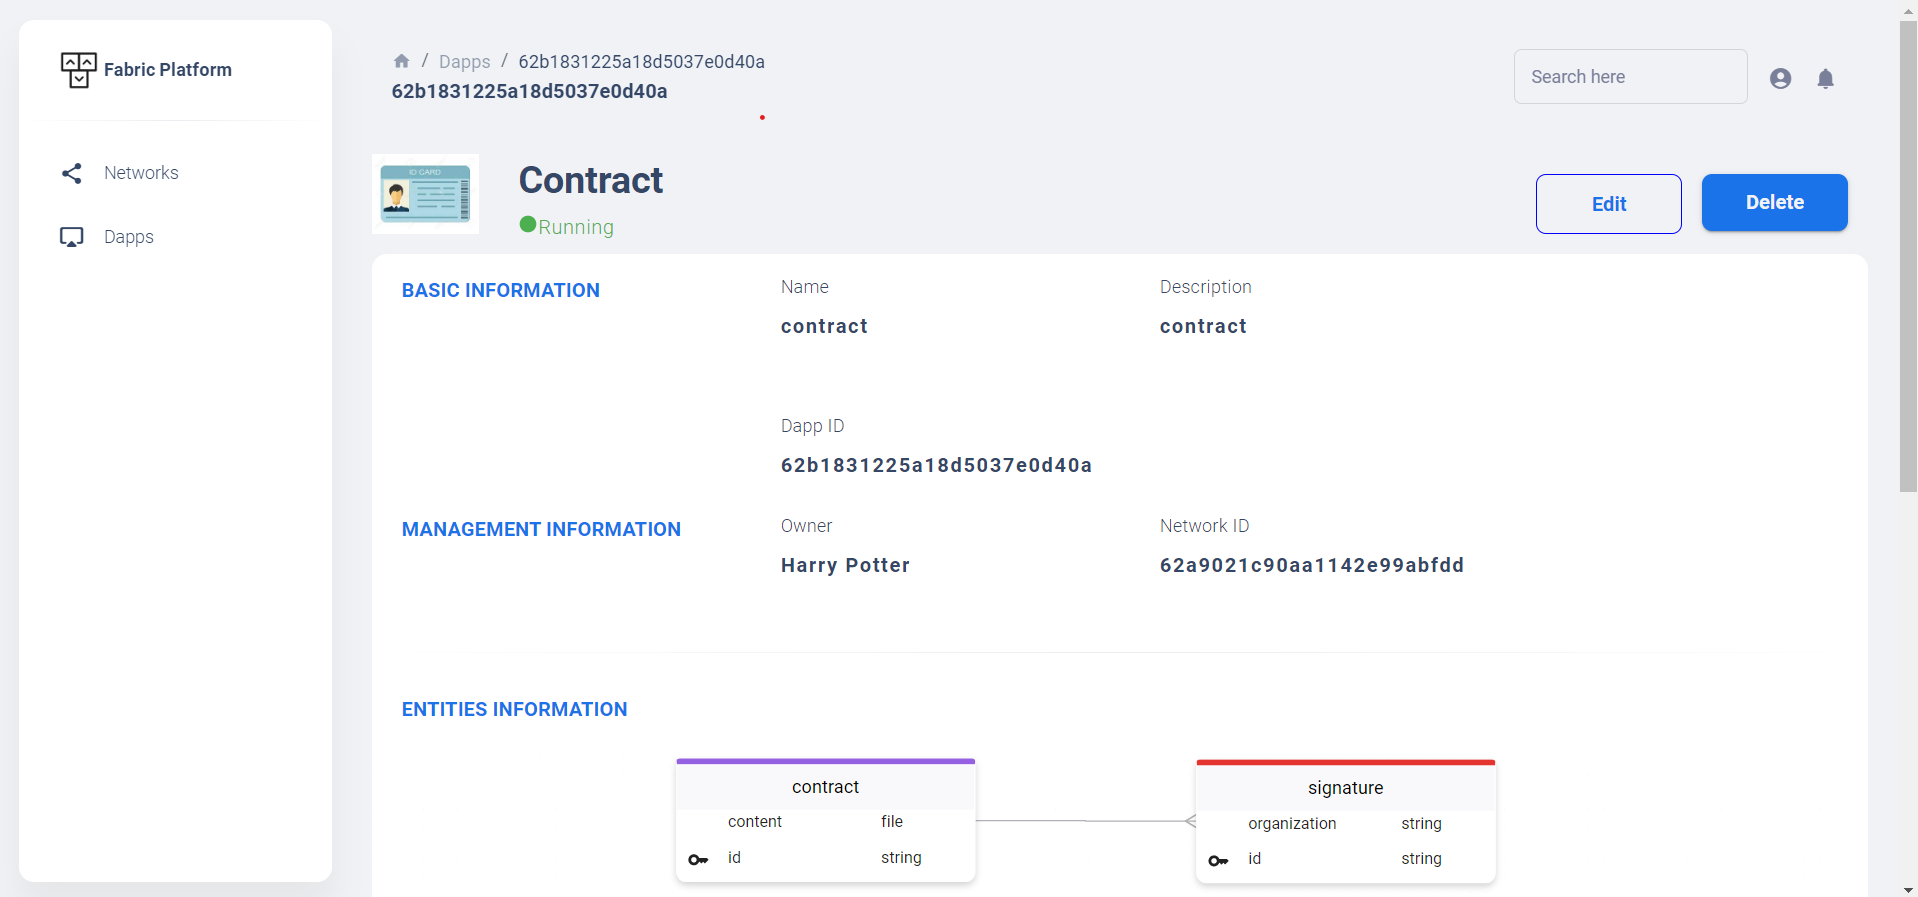
\includegraphics[width=0.75\linewidth]{Hinhve/DoAn-ResultDappDetail.png}
    \caption{Màn hình thông tin ứng dụng}
    \label{fig:ResultDappDetail}
\end{figure}

Hình \ref{fig:ResultDappDetail} mô tả màn hình thông tiết chi tiết của ứng
dụng. Ngoài thông tin, cấu trúc tổng quan của ứng dụng cũng được hiển thị.

\section{Kiểm thử}

\subsection{Kiểm thử hệ thống}

Để kiểm thử tác vụ tạo mạng và tạo ứng dụng phi tập trung mới, các tác vụ đó sẽ được thực hiện 10 lần và đo thời gian trung bình cần để hoàn thành các tác vụ đó. Kết quả được trình bày ở Bảng \ref{tab:TestNetwork} và \ref{tab:TestDapp}

\begingroup
\renewcommand{\arraystretch}{1.5} % Default value: 1
\begin{table}[H]
    \centering
    \def\arraystretch{1.5}
    \caption{Kết quả kiểm thử tác vụ tạo mạng}
    \label{tab:TestNetwork}
    \begin{tabular}{|p{0.3\textwidth}|p{0.525\textwidth}|}
        \hline
        Test Case ID                                       & TC1-1                                      \\ \hline
        Tác vụ                                             & Tạo mạng                                   \\ \hline
        Mô tả                                              & Đo thời gian tạo mạng trung bình           \\ \hline
        \multirow[t]{3}{0.3\textwidth}{Dữ liệu kiểm thử}   & Số máy ảo: 3                               \\
                                                           & Số tổ chức: 3 tổ chức mỗi tổ chức 3 peer   \\
                                                           & Cấu hình máy ảo: 4GB Ram, 2 vCpus          \\ \hline
        Điều kiện tiền đề                                  & Đã đăng nhập                               \\ \hline
        \multirow[t]{3}{0.3\textwidth}{Các bước thực hiện} & Bước 1: Đăng nhập                          \\
                                                           & Bước 2: Chạy kiểm thử với dữ liệu kiểm thử \\
                                                           & Bước 3: Lưu kết quả                        \\ \hline
        Kết quả mong muốn                                  & Thời gian tạo mạng trung bình: 900 giây    \\ \hline
        Kết quả thực tế                                    & Thời gian tạo mạng trung bình: 857 giây    \\ \hline
    \end{tabular}
\end{table}
\endgroup

\begingroup
\renewcommand{\arraystretch}{1.5} % Default value: 1
\begin{table}[H]
    \centering
    \def\arraystretch{1.5}
    \caption{Kết quả kiểm thử tác vụ tạo ứng dụng phi tập trung}
    \label{tab:TestDapp}
    \begin{tabular}{|p{0.3\textwidth}|p{0.525\textwidth}|}
        \hline
        Test Case ID                                       & TC1-2                                       \\ \hline
        Tác vụ                                             & Tạo ứng dụng                                \\ \hline
        Mô tả                                              & Đo thời gian tạo ứng dụng trung bình        \\ \hline
        \multirow[t]{3}{0.3\textwidth}{Dữ liệu kiểm thử}   & Một ứng dụng có 3 thực thể                  \\ \hline
        Điều kiện tiền đề                                  & Đã đăng nhập                                \\ \hline
        \multirow[t]{3}{0.3\textwidth}{Các bước thực hiện} & Bước 1: Đăng nhập                           \\
                                                           & Bước 2: Chạy kiểm thử với dữ liệu kiểm thử  \\
                                                           & Bước 3: Lưu kết quả                         \\ \hline
        Kết quả mong muốn                                  & Thời gian tạo ứng dụng trung bình: 200 giây \\ \hline
        Kết quả thực tế                                    & Thời gian tạo ứng dụng trung bình: 201 giây \\ \hline
    \end{tabular}
\end{table}
\endgroup

\subsection{Kiểm thử SDK}

\begin{figure}[H]
    \centering
    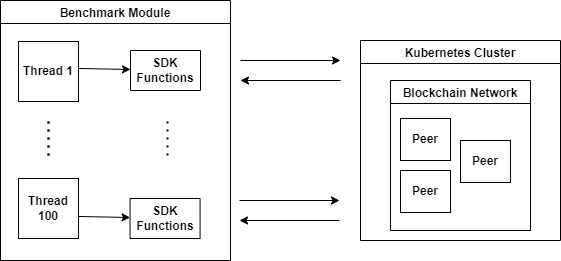
\includegraphics[width=0.75\linewidth]{Hinhve/DoAn-TestSDK.png}
    \caption{Mô-đun kiểm thử SDK}
    \label{fig:TestSDK}
\end{figure}

Hình \ref{fig:TestSDK} mô tả mô-đun sử dung để kiểm thử SDK. Mô-đun có thể gọi
đồng thời các hàm của SDK trên nhiều luồng.

\begin{figure}[H]
    \centering
    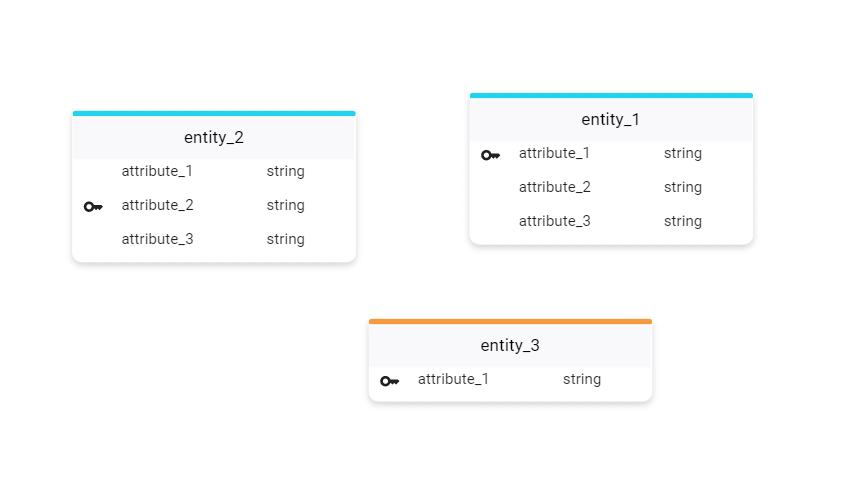
\includegraphics[width=0.75\linewidth]{Hinhve/DoAn-TestSDKDapp.png}
    \caption{Cấu trúc ứng dụng để kiểm thử SDK}
    \label{fig:TestSDKDapp}
\end{figure}

Để kiểm thử SDK, trước tiên tải về SDK của một ứng dụng có cấu trúc như hình \ref{fig:TestSDKDapp}. Tiếp đó sử dụng mô-đun kiểm thử SDK ở hình \ref{fig:TestSDKDapp} để giả lập việc gọi đồng thời các hàm trong SDK 100 lần rồi đo thời gian cần để hoàn thành tất cả 100 lần gọi đó. Kết quả kiểm thử được mô tả ở Bảng \ref{tab:TestSDKRead} và \ref{tab:TestSDKWrite}.

\begingroup
\renewcommand{\arraystretch}{1.5} % Default value: 1
\begin{table}[H]
    \centering
    \def\arraystretch{1.5}
    \caption{Kết quả kiểm thử các tác vụ đọc dữ liệu sử dụng SDK}
    \label{tab:TestSDKRead}
    \begin{tabular}{|p{0.3\textwidth}|p{0.525\textwidth}|}
        \hline
        Test Case ID                                       & TC2-1                                           \\ \hline
        Tác vụ                                             & Đọc dữ liệu từ Sổ cái sử dụng SDK               \\ \hline
        Mô tả                                              & Đo thời gian đọc dữ liệu sử dụng SDK trung bình \\ \hline
        Điều kiện tiền đề                                  & Đã đăng nhập                                    \\ \hline
        \multirow[t]{3}{0.3\textwidth}{Các bước thực hiện} & Bước 1: Tải SDK                                 \\
                                                           & Bước 2: Chạy mô-đun kiểm thử cho các hàm đọc    \\
                                                           & Bước 3: Lưu kết quả                             \\ \hline
        \multirow[t]{2}{0.3\textwidth}{Kết quả mong muốn}  & Tất cả các lần gọi hàm đều thành công           \\
                                                           & Tổng thời gian gọi: 1 giây                      \\ \hline
        \multirow[t]{3}{0.3\textwidth}{Kết quả thực tế}    & Tất cả các lần gọi hàm đều thành công           \\
                                                           & Tổng thời gian gọi: 0.41 giây                   \\
                                                           & Thời gian trung binh 1 lần gọi: 0.004 giây      \\ \hline
    \end{tabular}
\end{table}
\endgroup

\begingroup
\renewcommand{\arraystretch}{1.5} % Default value: 1
\begin{table}[H]
    \centering
    \def\arraystretch{1.5}
    \caption{Kết quả kiểm thử các tác vụ ghi dữ liệu sử dụng SDK}
    \label{tab:TestSDKWrite}
    \begin{tabular}{|p{0.3\textwidth}|p{0.525\textwidth}|}
        \hline
        Test Case ID                                       & TC1-2                                           \\ \hline
        Tác vụ                                             & Tạo ứng dụng                                    \\ \hline
        Mô tả                                              & Đo thời gian ghi dữ liệu sử dụng SDK trung bình \\ \hline
        Điều kiện tiền đề                                  & Đã đăng nhập                                    \\ \hline
        \multirow[t]{3}{0.3\textwidth}{Các bước thực hiện} & Bước 1: Tải SDK                                 \\
                                                           & Bước 2: Chạy mô-đun kiểm thử cho các hàm ghi    \\
                                                           & Bước 3: Lưu kết quả                             \\ \hline
        \multirow[t]{2}{0.3\textwidth}{Kết quả mong muốn}  & Tất cả các lần gọi hàm đều thành công           \\
                                                           & Tổng thời gian gọi: 2 giây                      \\ \hline
        \multirow[t]{3}{0.3\textwidth}{Kết quả thực tế}    & Tất cả các lần gọi hàm đều thành công           \\
                                                           & Tổng thời gian gọi: 1.62 giây                   \\
                                                           & Thời gian trung binh 1 lần gọi: 0.016 giây      \\ \hline
    \end{tabular}
\end{table}
\endgroup

Kết quả kiểm thử cho thấy hệ thống hoạt động ổn định. Các yêu cầu tạo mạng và
ứng dụng đều được xử lý thành công. Các tác vụ tương tác với mạng chuỗi khối
thông qua SDK nhanh và chính xác.

\section{Ứng dụng của hệ thống}

Để chứng minh mạng và SDK có thể được ứng dụng vào các nghiệp vụ thực tế, tôi đã xây dựng một ứng dụng web đơn giản tương tác với mạng và ứng dụng phi tập trung được tạo bởi hệ thống. Ứng dụng được gọi tên là Fabric Contract.

\subsection{Tổng quan ứng dụng}

Fabric Contract giải quyết bài toán sử dụng công nghệ chuỗi khối để số hóa và
minh bạch hóa quá trình ký hợp đồng giữa các doanh nghiệp, tổ chức. Công nghệ
chuỗi khối được sử dụng như một bằng chứng không thể chối cãi việc các bên liên
đã đồng ý và ký vào một hợp đồng cụ thể nào đó.

Cụ thể ứng dụng cho phép một tổ chức tạo một hợp đồng dưới định dạng tệp tin
pdf. Đại diện của các tổ chức sẽ thể hiện sự đồng thuận của mình với hợp đồng
đó bằng cách ký lên hợp đồng đó. Các tác vụ tạo, ký hợp đồng sẽ được lưu trữ
lên trên mạng chuỗi khối.

\subsection{Cấu hình}

Mạng mà ứng dụng sử dụng có cấu hình như Hình
\ref{fig:ContractAppNetworkConfig}

\begin{figure}[H]
    \centering
    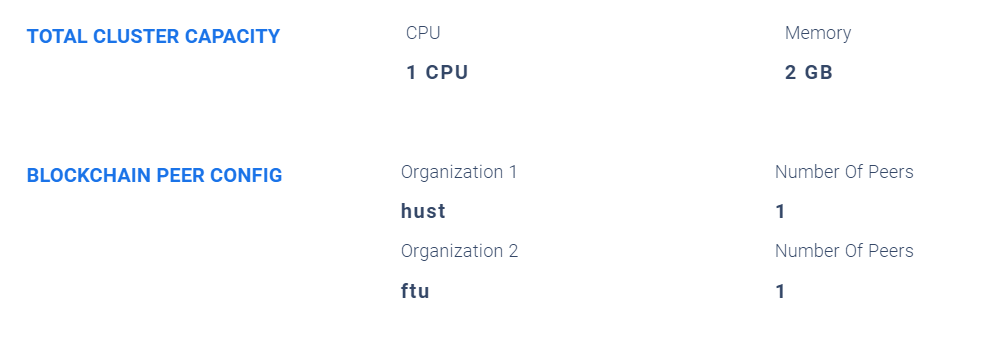
\includegraphics[width=0.75\linewidth]{Hinhve/DoAn-ContractAppNetworkConfig.png}
    \caption{Cấu hình mạng triển khai Fabric Contract}
    \label{fig:ContractAppNetworkConfig}
\end{figure}

Fabric Contract sẽ được sử dụng trong tác vụ tạo và ký hợp đồng giữa 2 tổ chức
trong mạng.

Ứng dụng phi tập trung mà Fabric Contract sử dụng có cấu hình như Hình \ref{fig:ContractDappConfig}

\begin{figure}[H]
    \centering
    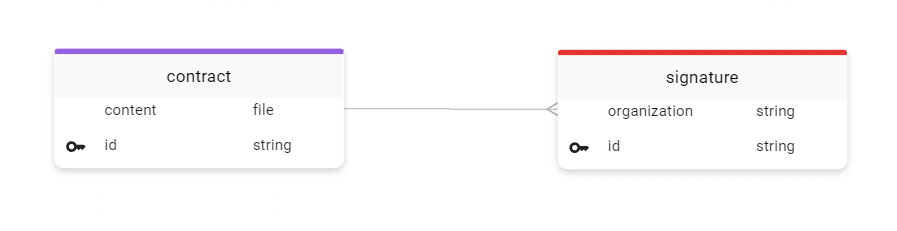
\includegraphics[width=0.75\linewidth]{Hinhve/DoAn-ContractAppDappConfig.png}
    \caption{Cấu hình mạng triển khai Fabric Contract}
    \label{fig:ContractAppDappConfig}
\end{figure}

Dữ liệu được lưu trữ trên mạng chuỗi khối bao gồm nội dung hợp đồng và các chữ
ký từ các tổ chức của hợp đồng đó. Từ các thông tin này có thể đảm bảo một hợp
đồng thực sự đã được chấp thuận bởi các bên liên quan.

\subsection{Luồng hoạt động}

\subsubsection{Tạo hợp đồng}

\begin{figure}[H]
    \centering
    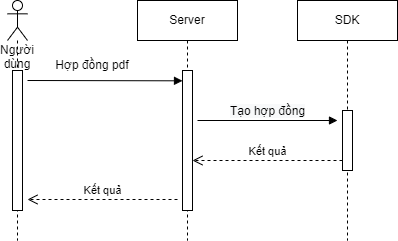
\includegraphics[width=0.75\linewidth]{Hinhve/DoAn-SeqCreateContract.drawio.png}
    \caption{Luồng tạo hợp đồng của Fabric Contract}
    \label{fig:SeqCreateContract}
\end{figure}

Hình \ref{fig:SeqCreateContract} mô tả luồng tạo hợp đồng của ứng dụng Fabric
Contract. Người dùng tải lên một tệp tin pdf tới Server. Server sử dụng SDK sẽ
tiến hành tạo một hợp đồng mới tương ứng với tệp tin đó và ghi dữ liệu lên mạng
chuỗi khối.

\subsubsection{Ký hợp đồng}

\begin{figure}[H]
    \centering
    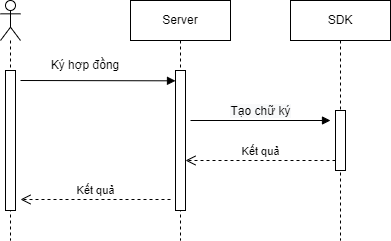
\includegraphics[width=0.75\linewidth]{Hinhve/DoAn-SeqSignContract.drawio.png}
    \caption{Luồng ký hợp đồng của Fabric Contract}
    \label{fig:SeqSignContract}
\end{figure}

Hình \ref{fig:SeqSignContract} mô tả luồng tạo hợp đồng của ứng dụng Fabric
Contract. Người dùng đại diện cho một tổ chức gửi yêu cầu ký hợp đồng tới
Server. Server sử dụng SDK sẽ tiến hành tạo một chữ ký mới cho hợp đồng đó và
cũng ghi dữ liệu lên mạng chuỗi khối.

\subsection{Minh họa hoạt động}

\begin{figure}[H]
    \centering
    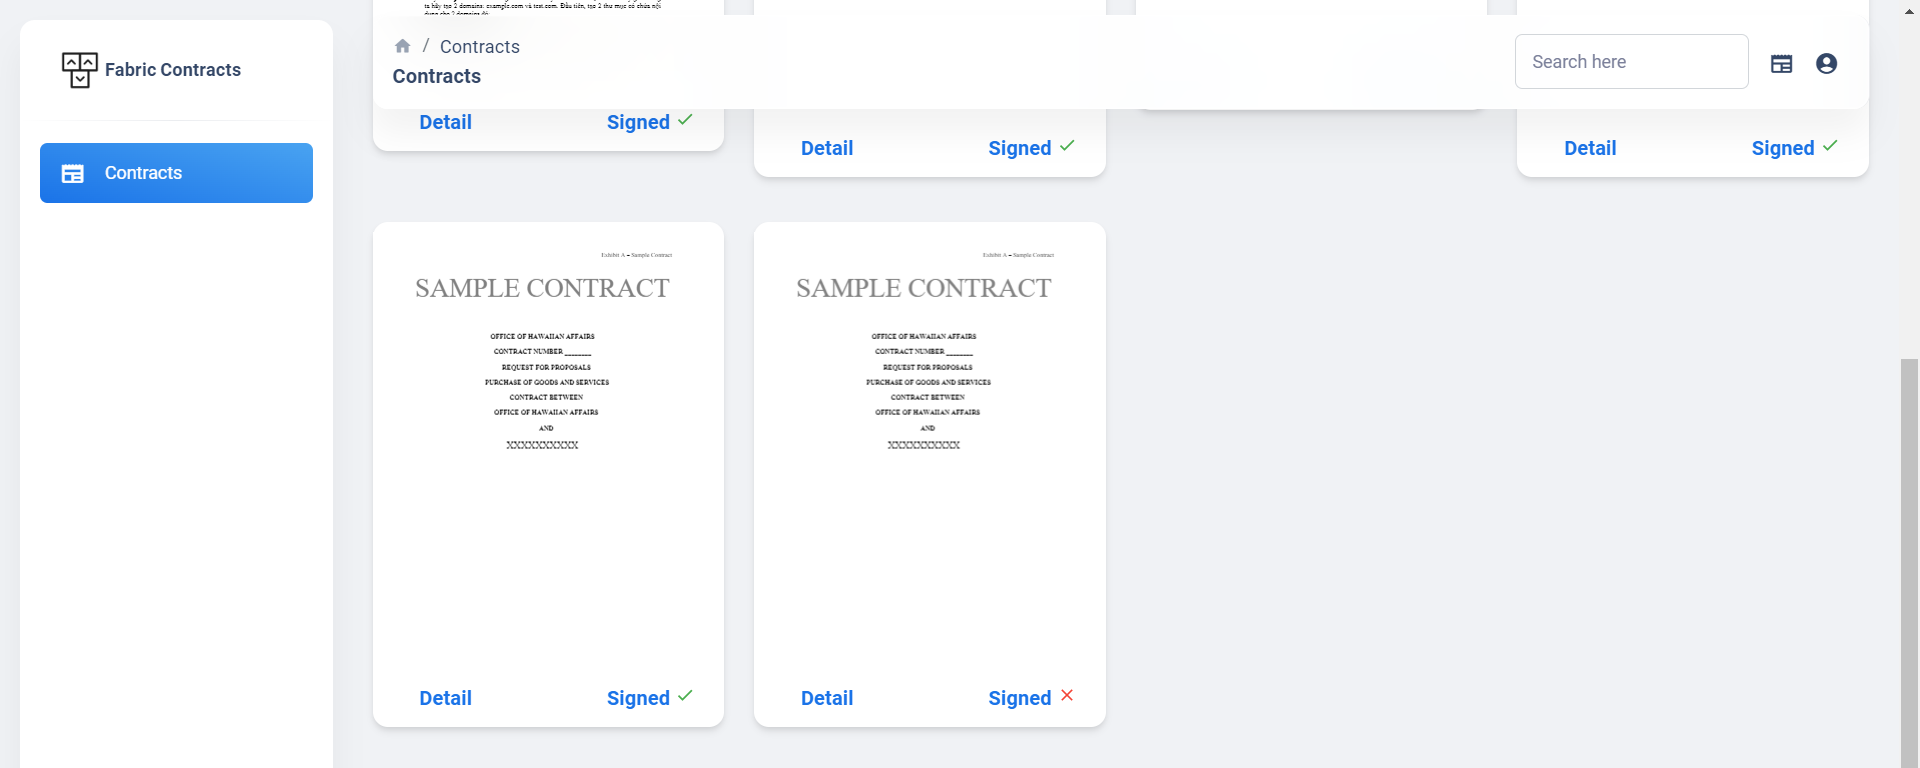
\includegraphics[width=0.75\linewidth]{Hinhve/DoAn-ScreenContracts.png}
    \caption{Màn hình danh sách hợp đồng Fabric Contract}
    \label{fig:ScreenContracts}
\end{figure}

Hình \ref{fig:ScreenContracts} mô tả danh sách các hợp đồng đã được tạo và
trạng thái hợp đồng đã được ký bởi hai bên hay chưa.

\begin{figure}[H]
    \centering
    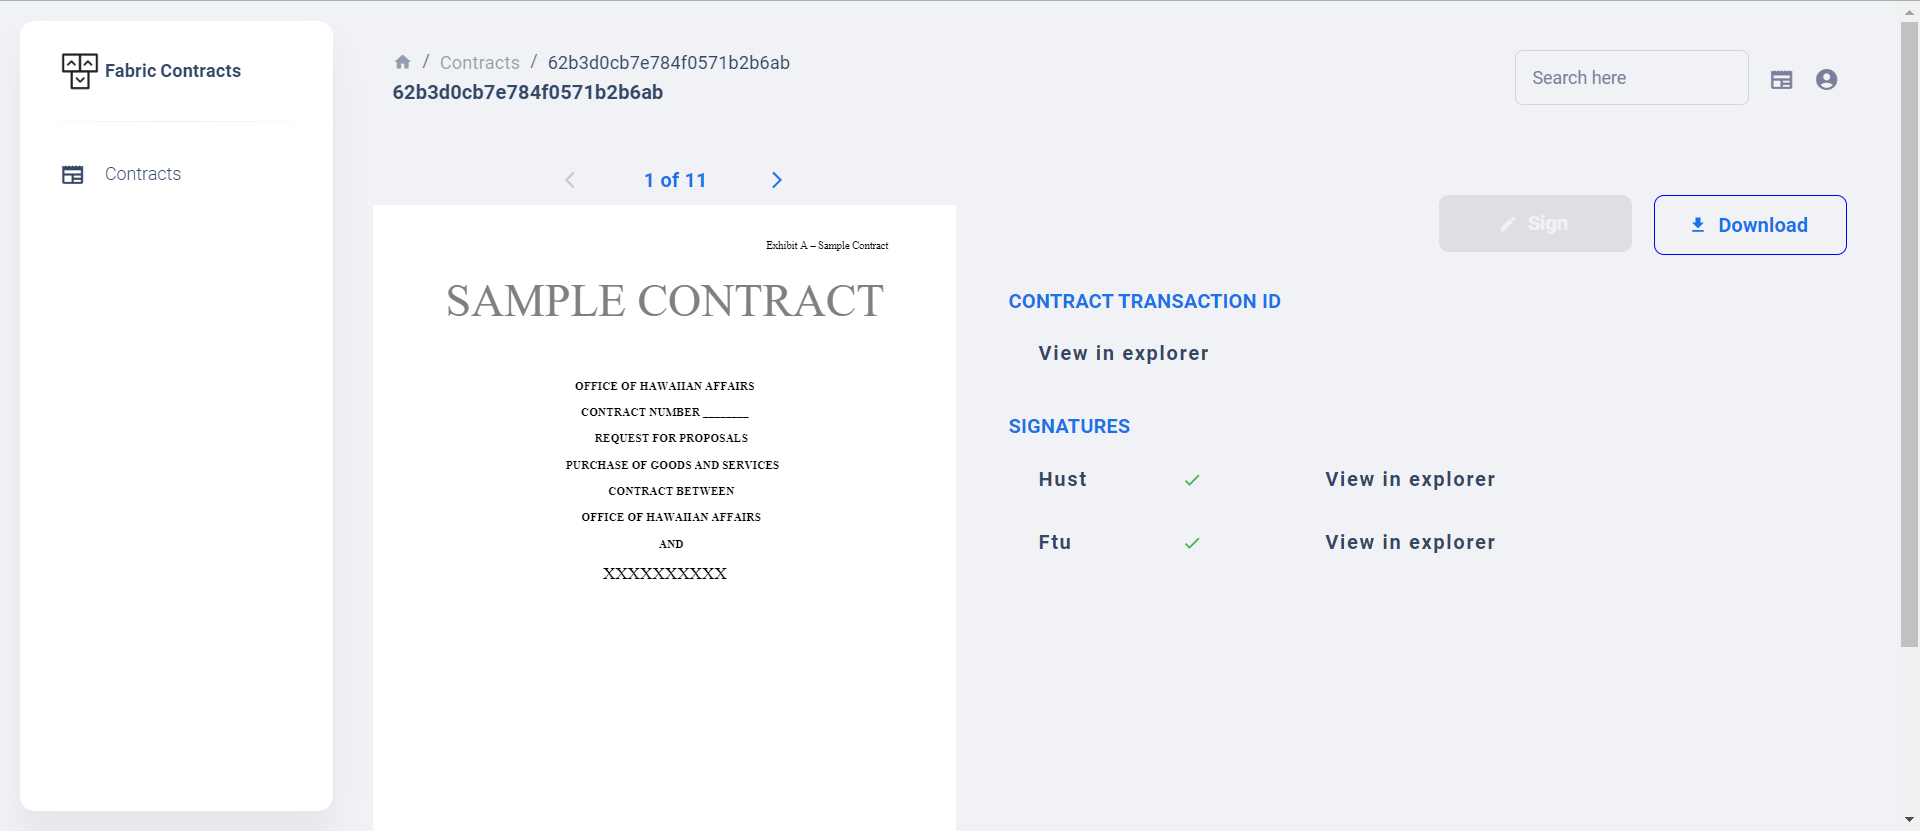
\includegraphics[width=0.75\linewidth]{Hinhve/DoAn-ScreenContractDetail.png}
    \caption{Màn hình chi tiết hợp đồng Fabric Contract}
    \label{fig:ScreenContractDetail}
\end{figure}

Hình \ref{fig:ScreenContractDetail} mô tả mà hình chi tiết của một hợp đồng.
Người dùng có thể thực hiện tác vụ ký tại màn hình này. Ngoài ra, người dùng có
thể xem chi tiết các giao dịch trên mạng chuỗi khối liên quan đến việc tạo và
ký hợp đồng này.

\begin{figure}[H]
    \centering
    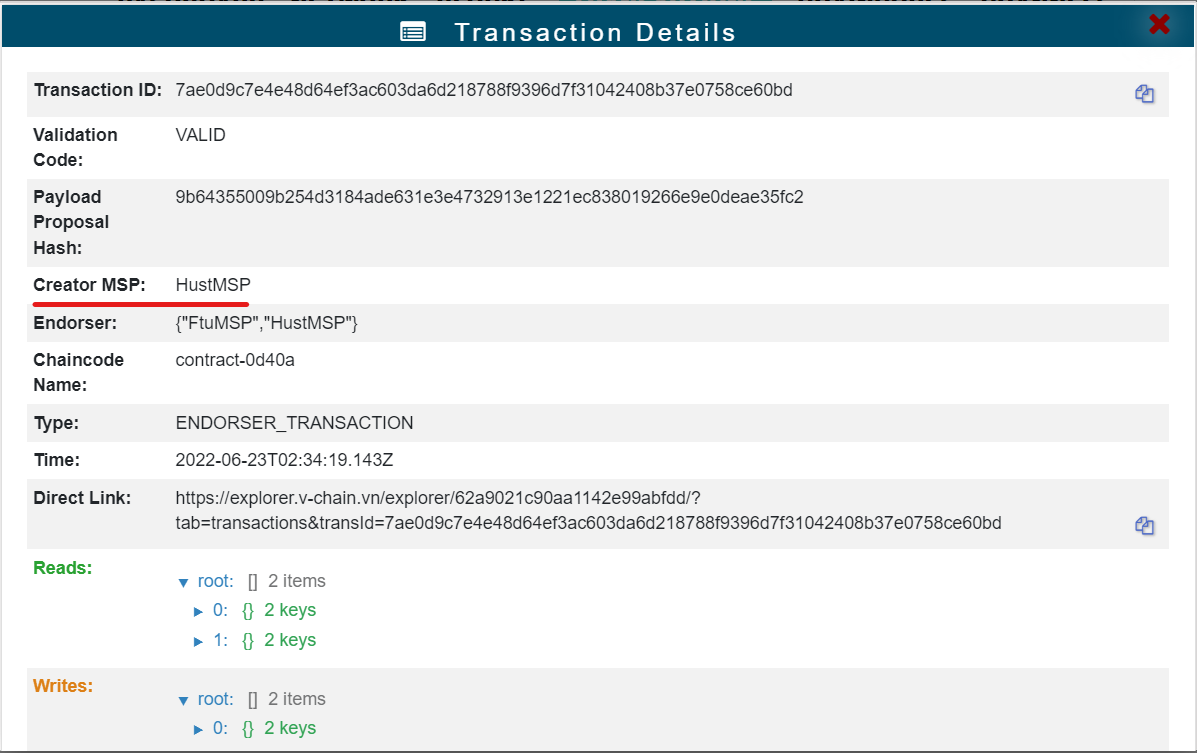
\includegraphics[width=0.75\linewidth]{Hinhve/DoAn-ExplorerContract.png}
    \caption{Giao dịch ký hợp đồng trên mạng chuỗi khối}
    \label{fig:ExplorerContract}
\end{figure}

Hình \ref{fig:ExplorerContract} mô tả thông tin về giao dịch để ký hợp đồng
được xem thông qua ứng dụng Explorer của mạng Hyperledger Fabric. Có thể thấy
rõ thông tin của tổ chức tạo giao dịch này thông qua CreatorMSP. Thông tin này
sẽ được sử dụng để chứng minh một tổ chức đã chấp thuận và ký lên một hợp đồng. % \section{Triển khai}
% Sinh viên trình bày mô hình và/hoặc cách thức triển khai thử nghiệm/thực tế.
% Ứng dụng của sinh viên được triển khai trên server/thiết bị gì, cấu hình như
% thế nào. Kết quả triển khai thử nghiệm nếu có (số lượng người dùng, số lượng
% truy cập, thời gian phản hồi, phản hồi người dùng, khả năng chịu tải, các thống
% kê, v.v.)

Chương 5 đã trình bày về chi tiết thiết kế xây dựng cũng như quá trình kiểm thử
đánh giá hệ thống. Đây là cơ sở quan trọng để đi đến Chương 6, chương cuối
cùng.

\end{document}
